%%% 05-06-2015 updated from 30-04-2015 updated from 02-15-2015
%%% Post reviewers decision for NBA journals
\documentclass[12pt,a4paper]{article}
\newcommand{\myreferences}{C:/Users/Jaime/Documents/GitHub/bibliography-jgr/bibliojgr}
\usepackage{subfigure}

%\usepackage[hang]{footmisc}
%\pagenumbering{arabic}
%\setlength{\footnotemargin}{0pt}
%\usepackage{footmisc,multicol, graphicx,makeidx,courier,helvet}
\usepackage[T1]{fontenc}
\usepackage[]{inputenc}
\usepackage{amssymb,amsmath} 
\usepackage{amsfonts}
\usepackage{booktabs}

\usepackage{float}
\usepackage{graphicx}
\usepackage{epstopdf}
\usepackage{textcomp}  %for degree symbol
%\usepackage{apacite}
%\usepackage{babel}

\newcommand*{\addheight}[2][.5ex]{%
\raisebox{0pt}[\dimexpr\height+(#1)\relax]{#2}%
}
\usepackage{mathptmx}         % selects Times Roman as basic font
\usepackage{helvet}         % selects Helvetica as sans-serif font
\usepackage{courier}        % selects Courier as typewriter font
\usepackage{type1cm}        % activate if the above 3 fonts are
\usepackage{makeidx}         % allows index generation
\usepackage{graphicx}        % standard LaTeX graphics tool
\usepackage{multicol}        % used for the two-column index
\usepackage{array}
\usepackage{tabularx}
\usepackage[affil-it]{authblk}  %package for multiple authors
\usepackage{caption}
\graphicspath{{C:/Users/Jaime/Documents/GitHub/figures/}}
\makeindex   

\title{A quantitative study of network robustness in resting state fMRI in young and elder conditions}
\author[1]{Jaime Gomez-Ramirez\thanks{Corresponding author \hspace{0.6cm} jaime.gomez-ramirez@sickkids.ca}}
\author[2]{Yujie Li}%\thanks{liyj596@mail.ccnu.edu.cn}}
\author[3]{Qiong Wu}%\thanks{gen421111@s.okayama-u.ac.jp}}
%\author[3]{Xiaoyu Tang\thanks{D.D@university.edu}}
\author[3]{Jinglong Wu}%\thanks{wu@mech.okayama-u.ac.jp}}
\affil[1]{The Hospital for Sick Children, Department of Neuroscience and Mental Health, University of Toronto, Bay St. 686, Toronto, Canada}
\affil[2]{Key Laboratory of Adolescent Cyberpsychology and Behavior (CCNU), Ministry of Education, Wuhan 430079, China and School of Psychology, Central China Normal University, Wuhan 430079, China}
\affil[3]{Biomedical Engineering Laboratory, Okayama University, 1-1-1 Tsushima-naka, Kita-ku, Okayama, Japan and Intelligent Robotics Institute, School of Mechatronics Engineering,Beijing Institute of Technology, Beijing, China}
\renewcommand\Authands{ and }

\begin{document}
\def\s{\sigma}
\date{}
\maketitle

\abstract{
Brain connectivity analysis have shown great promise in understanding of how aging affects   
functional connectivity, however, an explanatory framework to study healthy aging in terms of network efficiency is still missing. Here we study network robustness i.e., resilience to
perturbations, in resting state functional connectivity networks (rs-fMRI) in young and elder subjects. 
We apply analytic measures of network communication efficiency in the human brain to make reasonable guesses about  compensatory mechanisms elicited in aging. 
Specifically, we quantify the effect of "lesioning" (node cancelling) of either single regions-of-interest (ROI) or whole networks on global connectivity metrics  (i.e., efficiency).
We find that young individuals are more resilient than old ones to random "lesioning" of brain areas, global network efficiency is over 3 times lower in older subjects relative to younger subjects. On the other hand, the "lesioning" of central and limbic structures in young subjects yield a larger efficiency loss than in older individuals. Overall our study shows a more idiosyncratic response to specific brain network "lesioning" in elder compared to young subjects, and that young adults are more resilient to random deletion of single nodes compared to old adults.}
%The main finding was that the effects of node cancelling were very different in each group. For this purpose, they evaluated the amount of global efficiency before and after this 'functional intervention'.
%Then, they investigated the effect of zeroing some nodes or entire subnetworks from the whole brain.
%We investigate the effect of the lesioning of either indiviudual brain regions and networks of regions in young and elder subjects. 
%Resiliency in elder is network specific 
%\keywords{resting state fMRI, network degeneration hypothesis, Markov chain,
%relative entropy}

\section{Introduction}
%i.Relevance of RS 
It has been suggested that fluctuations in the BOLD\footnote{Blood-oxygen-level dependent contrast imaging is the method used in functional magnetic resonance imaging (fMRI) to determine which parts of the brain are most active.} signal measured
in humans in resting state represent the neuronal activity baseline and shape
spatially consistent patterns \cite{Raichle:2005}, \cite{Fransson:2006}. The 
slow fluctuations in the BOLD signal found in resting subjects are highly
coherent within either structural or functional networks in the human brain.
Functional correlation based on the synchrony of low-frequency blood flow
fluctuations in resting state have been identified in the sensorimotor
\cite{kokkonen_preoperative_2009}, visual \cite{damoiseaux_consistent_2006},
language \cite{hampson_detection_2002}, auditory
\cite{hunter_neural_2006} and attention
\cite{fox_spontaneous_2006} and the frontoparietal control system
\cite{vincent_evidence_2008}.

%ii.Approaches 
The visual identification of the
overall connectivity patterns in resting state functional magnetic resonance
imaging (rs-fMRI), has been assessed first and foremost using both model-based and model-free
approaches. The former, uses voxel-wise analysis of brain images to build statistical parametric maps of brain activation \cite{biswal_functional_1995}. 
While this approach has been successful in, for instance, 
the identification of motor networks \cite{robinson_resting_2009}, it shows important limitations when
the seed voxel cannot be easily identified \cite{maldjian_functional_2001}.  
For example, in brain areas with unclear boundaries i.e., cognitive networks involved in memory or self processing operations \cite{fingelkurts_persistent_2011}. 
Independent Component Analysis (ICA), on
the other hand, is a model-free approach that allows separating resting
fluctuations from other signal variations, resulting in a collection of spatial
maps, one for each independent component, that represent functionally relevant networks in the brain
\cite{calhoun_review_2009}.
%Bad sentence, improve style
While ICA has the advantage over the parametric approach that it does not need to
assume a specific temporal model of correlation between regions of
interest, the functional relevance of the different components is, however,
computed relative to their resemblance to a number of networks, based on
criteria that are not easily formalized \cite{biswal_toward_2010}.

%Graph-based 3ra via 
A third approach, complementary to the other two, that is becoming of paramount importance is the network-based approach. Graph-based techniques provide new
insights into the structure function relationship in the healthy brain, aging and neuropathological disorders \cite{fair_functional_2009}, 
\cite{wang_graph-based_2010}, \cite{he_graph_2010}, \cite{wang_graph_2011}, \cite{yu_altered_2011}, \cite{brier_functional_2014}, \cite{sala-llonch_changes_2014}. 
The use of graph theoretic techniques to model brain networks has shifted the 
emphasis from the identification of local subnetworks -default mode network,
primary sensory motor network etc.- to the quantitative study of the topological
and informational characteristics of large-scale brain networks.
The quantitative analysis of complex networks have been rapidly adopted in the cognitive neuroscience community, linking graph theoretic metrics  to brain network organization \cite{bullmore_complex_2009}, \cite{sporns_contributions_2014},  specific behavioral abnormalities \cite{tschernegg_abnormalities_2013}, \cite{cocchi_functional_2012} and  clinical outcomes \cite{yuan_structural_2015}, \cite{anderson_abnormal_2013}, \cite{dickerson_large-scale_2009} . It is of note that notable proponents of a modularist vision of brain
connectivity to understand cognition, such as Gazzaniga
\cite{gazzaniga_new_1999}, \cite{Fuster:2000}, has
now embraced a "complex brain networks approach" \cite{bassett_understanding_2011}. 

Network-based approaches to rs-fMRI have demonstrated
non-trivial topological properties of functional networks in the human brain.
Large-scale anatomical
connectivity analysis in the mammalian brain, shows that brain topology is
neither random nor regular. Instead, small world
architectures \cite{Watts:1998} -highly clustered nodes connected thorough
relatively short paths- have been identified in brain networks. 
%\cite{Vaessen:2010}.
Small world networks are not solely
structural, functional networks with a small world organization have been
identified in the mammal brain \cite{Bassett:2006}. Small world network properties have also been consistently found across different
conditions, including normal development, aging, and
in various pathological conditions \cite{wang_graph-based_2010}, \cite{anderson_decreased_2013}, \cite{stam_modern_2014}. 
%http://www.ncbi.nlm.nih.gov/pmc/articles/PMC3604768/
While network-based studies have been successful in delineating generic network properties such as
path length or clustering, additional work is needed in order to come to grips
with the internal working of the systems.
Computational simulations of disruptions in the network
architecture of resting state can give clues about
normal development and pathological conditions. For example, Supekar and
colleagues \cite{Supekar:2008} have shown that the deterioration of small world
properties such as the lowering of the cluster coefficient, affect local
network connectivity, which in turn may work as a network biomarker for
Alzheimer's disease. Abnormalities in small-worldness may also have a
significant positive correlation in, for example, schizophrenia
\cite{liu_disrupted_2008} and epilepsy \cite{liao_altered_2010}, \cite{zhang_altered_2011}.

%Transport efficiency
Transport network efficiency measures have been used to study the relationship between structural and resting state functional connectivity \cite{goni_resting-brain_2014}. 
The effects of lesioning in white matter connections can be studied via the simulation of the removal of individual connections from the connectome. Irimia and Van Hornreport \cite{irimia_systematic_2014}, using this technique, have been able to delineate "a core scaffold" or white matter network connections that when disrupted, trigger dramatic changes in the overall organization of the human connectome.   

A systematic study of the effects of simulated lesioning in rs-fMRI is still missing. 
In this paper we try to fill this gap, providing efficiency and robustness measures to quantify the impact of simulated lesioning  based on \cite{latora_efficient_2001}.
Aging is a complex physiological process with multiple temporal and spatial scales and it is unrealistic to expect any all encompasing predictive model. However, a common finding is that older subjects present reduced functional connectivity compared to young adults. We will try to replicate this finding and go beyond, by identifying the brain networks that when disconnected from the rest of the brain, result in dramatic/mild efficiency loss in transmitting information. 
Previous studies have shown that modularity in both young and elderly condition is not random \cite{meunier_age-related_2009}, \cite{song_age-related_2014}. Nevertheless, a general picture of how normal aging affects network efficiency is missing. Here, we explore the hypothesis that normal aging brain is associated with changes in network efficiency. 
%We provide a metric to analyze how efficiency in functional connectivity is affected by aging. 
We investigate the hemispheric asymmetry reduction hypothesis, studying the effects of lesioning hemispheres separately in older compared to young adults.  

The rest of the paper is structured as follows. Section \ref{mat-methods} introduces the 
methodology followed in the data acquisition and reconstruction, data
pre-processing, and data connectivity analysis in the young and elder conditions. Then, we build a model to study quantitatively how network robustness is affected upon the removal of both nodes and specific networks as well as edges in both conditions. The simulations of the model are shown in Section \ref{results}. The empirical and clinical implications of the model are discussed in Section \ref{discussion}. 

\section{Materials and Methods}
\label{mat-methods}

\subsection{Data acquisition}

Forty-two healthy volunteers separated in two groups, twenty-three healthy young volunteers (ages 21-32; mean 22.7; male/female 23/0) and 19 healthy older volunteers (ages 60-78; mean 66.5; male/female 16/3; MMSE score 29.5 +- 0.1) took part in the fMRI experiment. All subjects had
normal or corrected-to-normal vision and all the participants in both conditions have not been diagnosed with mild cognitive impairment nor psychiatric or neurological disorders. 
The study was approved by the ethics
committee of Okayama University, and written informed consent was obtained before the study. All subjects were imaged using a 1.5 T Philips scanner vision whole-body MRI system (Okayama University Hospital, Okayama, Japan), which was equipped with a head coil. Functional MR images were acquired during rest when subjects were
 instructed to keep their eyes closed and not to think of anything in
 particular. The imaging area consisted of 32 functional gradient-echo planar
 imaging (EPI) axial slices (voxel size=3x3x4 mm3, TR=3000 ms, TE=50 ms,
 FA=90�, acquisition matrix=80�79, FOV=240�240 mm2, slice thickness=4 mm, gap=0.5 mm) that were used to obtain T2*-weighted fMRI images in the
 axial plane. We obtained 176 functional volumes and excluded the first 4 scans
 from analysis. After the EPI scan, a T1-weighted 3D magnetization-prepared
 rapid acquisition gradient echo (MP-RAGE) sequence was acquired (TR=9.4 ms, TE=4.6 ms, FA=10�, acquisition matrix=240�240, voxel size=1�1�1 mm3, 200 contiguous axial slices).

\subsection{Data preprocessing} 
Data were preprocessed using Statistical Parametric Mapping software SPM8
\footnote{http://www.fil.ion.ucl.ac.uk/spm/} and REST v1.7
\footnote{http://restfmri.net/forum/index.php}. To correct for differences in
slice acquisition time, all images were synchronized to the middle slice.
Subsequently, images were spatially realigned to the first volume due to head
motion. None of the subjects in both conditions had head movements exceeding 2.5 mm on any axis or
rotations greater than 2.5\textdegree. After the correction,  the imaging data were
normalized to the Montreal Neurological Institute (MNI) EPI template supplied
with SPM8 (resampled to 2x2x2 mm$3$ voxels) \footnote{http://imaging.mrc-cbu.cam.ac.uk/imaging/Templates}. In order to avoid introducing artificially local spatial correlation, the normalized images were
not smoothed. Finally, the resulting data were temporally band-pass filtered
(0.01-0.08 Hz) to reduce the effects of low-frequency drifts and high-frequency
physiological noises \cite{jiao_granger_2011}.

\subsection{Anatomical parcellation} 
Before whole brain parcellation, several sources of spurious variance including
the estimated head motion parameters, the global brain signal and the average
time series in the cerebrospinal fluid and white matter regions were removed
from the data through linear regression. It ought to be noted that Murphy and colleagues in \cite{murphy_impact_2009}  
have pointed out that global signal removal may artificially introduce anti-correlated networks. 
The effect of the removal of the global signal on resting state correlation maps have been examined by Fox and colleagues \cite{fox_global_2009}, reaching to the conclusion that several characteristics of anticorrelated networks are not attributable to global signal removal and therefore suggesting a biological basis for those anticorrelations.  
The fMRI data were parcellated into 90 regions using an automated anatomical labeling template (AAL) \cite{tzourio-mazoyer_automated_2002}. For each subject, the mean time series of each region was obtained by simply
averaging the time series of all voxels within that region.

\subsection{Brain network construction} 
To measure the functional connectivity among regions, we calculated the Pearson
correlation coefficients between any possible pair of regional time series, and
then obtained a temporal correlation matrix $(90x90)$ for each subject. We
applied Fisher's r-to-z transformation to improve the normality of the
correlation matrix. Then, two-tailed one-sample t-tests were performed for all
the possible $4005=\frac{90x89}{2}$ pairwise correlations across subjects
to examine whether each inter-regional correlation significantly differed from
zero. 
A Bonferroni-Holm correction for multiple comparisons was
further used to threshold the correlation matrix into an adjacency matrix M. $M(i,j) =1$ if there is a significant correlation between brain regions $i$ and $j$ and $M(i,j) =0$, otherwise (Figure \ref{fig:adjmat}). Finally, an undirected binary graph was acquired in which nodes represent brain regions and edges represent links between regions.

\subsection{Information Efficiency}
\label{ss:nrobeffvul}
%Distance related measures (Network Efficiency and Network Vulnerability)
A quantitative understanding of network robustness, that is, functional
network invariance under perturbation can shed light on 
the properties that mediate in developmental, aging and pathological processes
in the human brain. In essence, robustness measures the capacity of the network to
perform the same function before and after a perturbation. Perturbations are
events, internal or external, that elicit a change in the network
configuration. Possible perturbations are the obliteration of one or more nodes and changes in the
connectivity between nodes. 
%Here we perform perturbations that consist on the obliteration of one or more nodes together with and all the edges that connect the lesioned node.

The efficiency of a network is a network centrality
measure that quantifies the network's reliability in transmitting information. It follows that the  efficiency loss after the removal of a
node or a set of nodes is the normalized difference in network efficiency before and after the intervention.
Latora and Marchiori \cite{latora_efficient_2001} proposed a measure of network
efficiency defined as the efficiency in transmitting information 
between any two nodes $(i,j)$ in a graph G as the inverse of the shortest path that
connects them
\begin{equation}
\varepsilon_{ij}= \frac{1} {d_{ij}}
\label{eq:geod}
\end{equation}
where $d_{ij}$ is the
shortest path length or the geodesic distance between nodes $i$ and $j$. 
Note that when there is no path that connects the nodes i and j, $d_{ij}=
\infty$, and the efficiency in the communication of the two nodes is zero,
$\varepsilon_{ij}=0$.

The efficiency of the network G, $\Sigma(G)$, is then calculated as the average of the efficiency
between any two nodes $\varepsilon_{ij}$ 
\begin{equation}
\Sigma(G)=\frac{\sum_{i \neq j} \varepsilon_{ij}} {N(N-1)}
=\frac{1}{N(N-1)}\frac{1}{\sum_{i \neq j } d_{ij}}
\label{eq:latm}
\end{equation}
where $N$ is the number of nodes. 
 
We can calculate
the information centrality $C$ of any node i in a network G as the variation
in the network efficiency caused by the removal of the edges incident in i. Thus, the
information centrality of a node i, $C_i$, is the difference between the
efficiency of the original network G with N nodes and E edges, $G(N,E)$, and the
efficiency of the resulting graph $G(N-i,E-k_i)$ with $N-i$ nodes and $E-k_i$ edges, where
$k_i$ denotes the set of edges incident to node i. The centrality of a
node is a normalized measure of the loss in network efficiency, caused by the isolation of a node in G. Formally,

\begin{equation}
C_i=\frac {\Sigma(G(N,E)) - \Sigma(G(N-i,E-k_i))} {\Sigma(G(N,E))} 
\label{eq:centr}
\end{equation}

From equation \ref{eq:centr}, a network $G$ is considered to be robust to
a perturbation if the network efficiency, $\Sigma(G)$, 
stays close to the original value after a perturbation. Ideally $\Sigma(G(N,E)) = \Sigma(G(N -i,E-k_i))$
with efficiency loss or centrality of node i equals to 0.
By the same token, the information centrality of a set of nodes $S$ or the efficiency loss upon the removal of $S$, can be calculated as the normalized measure of the loss in network efficiency caused by the isolation of a set of nodes S in G.

\begin{equation}
C_S=\frac {\Sigma(G(N,E)) - \Sigma(G(N-S,E-k_S)) } {\Sigma(G(N,E))} 
\label{eq:centrS}
\end{equation}

\section{Results}
\label{results}

% random 
 The global network efficiency for unperturbed networks as defined in Equation \ref{eq:latm} is
 0.3678 for young subjects and 0.1144 for elder subjects. Thus, young subjects
 connectivity network is a bit more than three times more efficient in terms of the shortest
 path distance between any two nodes \ref{fig:adjmat}.

In order to obtain the efficiency measures described in Equations \ref{eq:centr} and \ref{eq:centrS}, we perturb the resting state network in three ways. First, using random single node deletion (Section \ref{ss:single}),  second targeting specific networks of interest (Section \ref{ss:target}) and third the efficiency loss after lesioning edges (Section \ref{ss:edges}). 

\begin{figure}[H]
    \subfigure[\label{subfig-1:dummy}]{%
      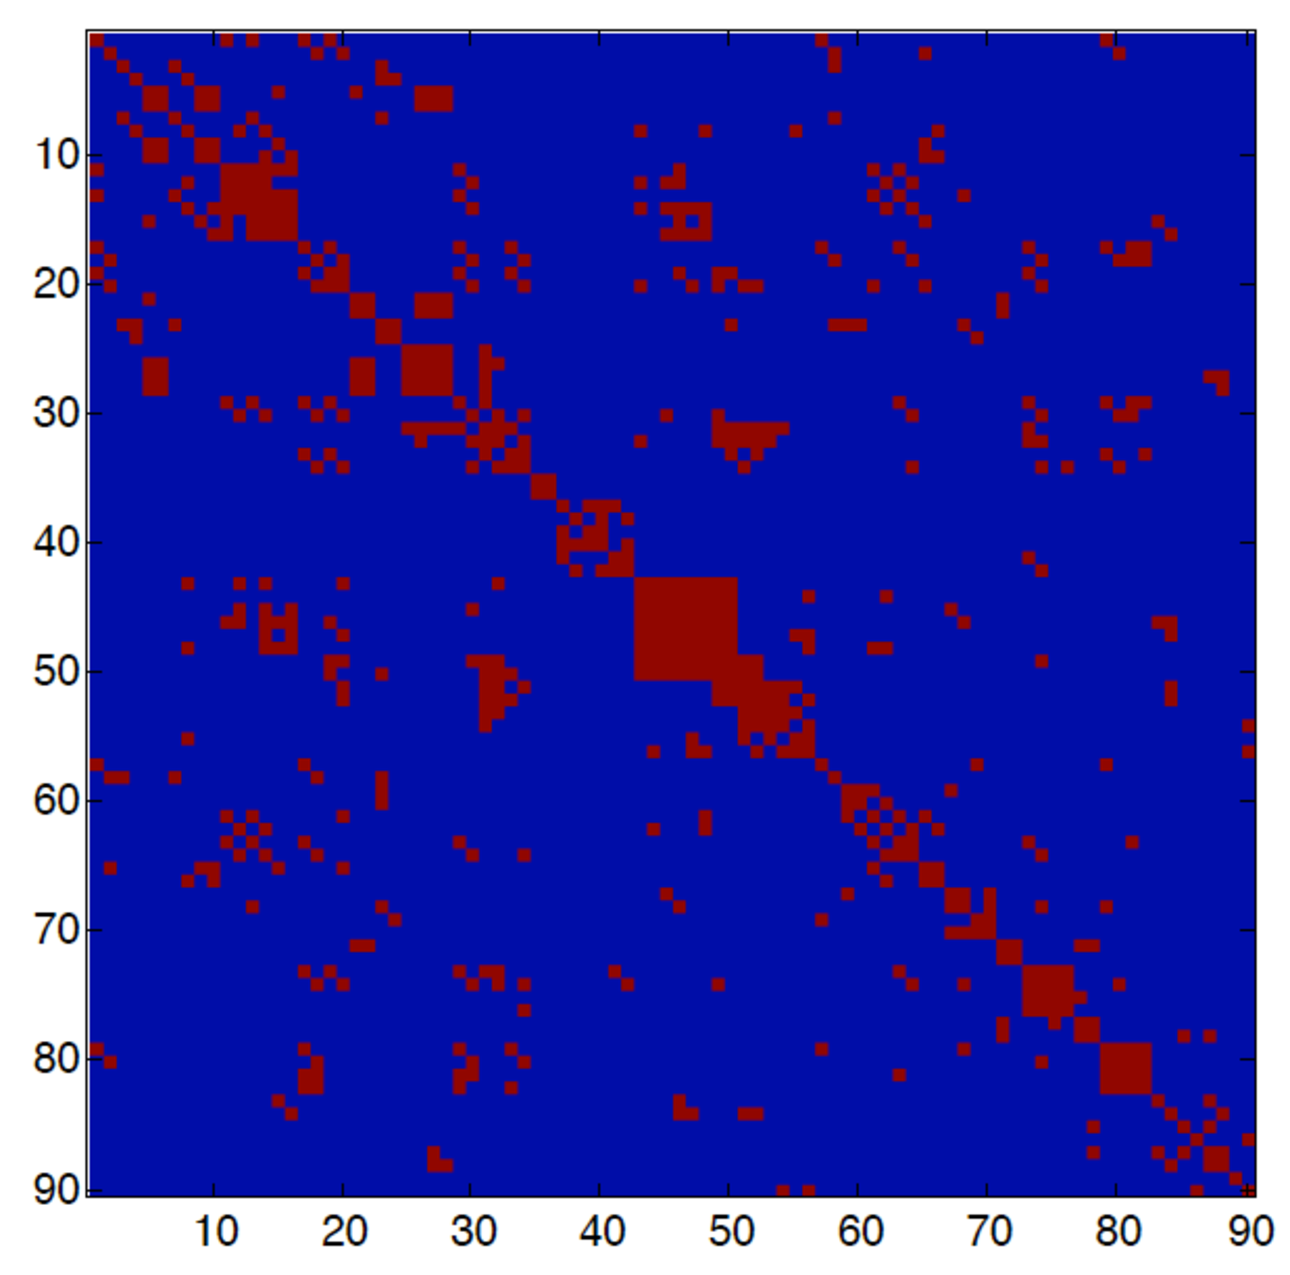
\includegraphics[width=0.5\textwidth,height=0.5\textheight,keepaspectratio]{figures/youngadjmatrix.pdf}
    }
    \hfill
    \subfigure[\label{subfig-2:dummy}]{%
      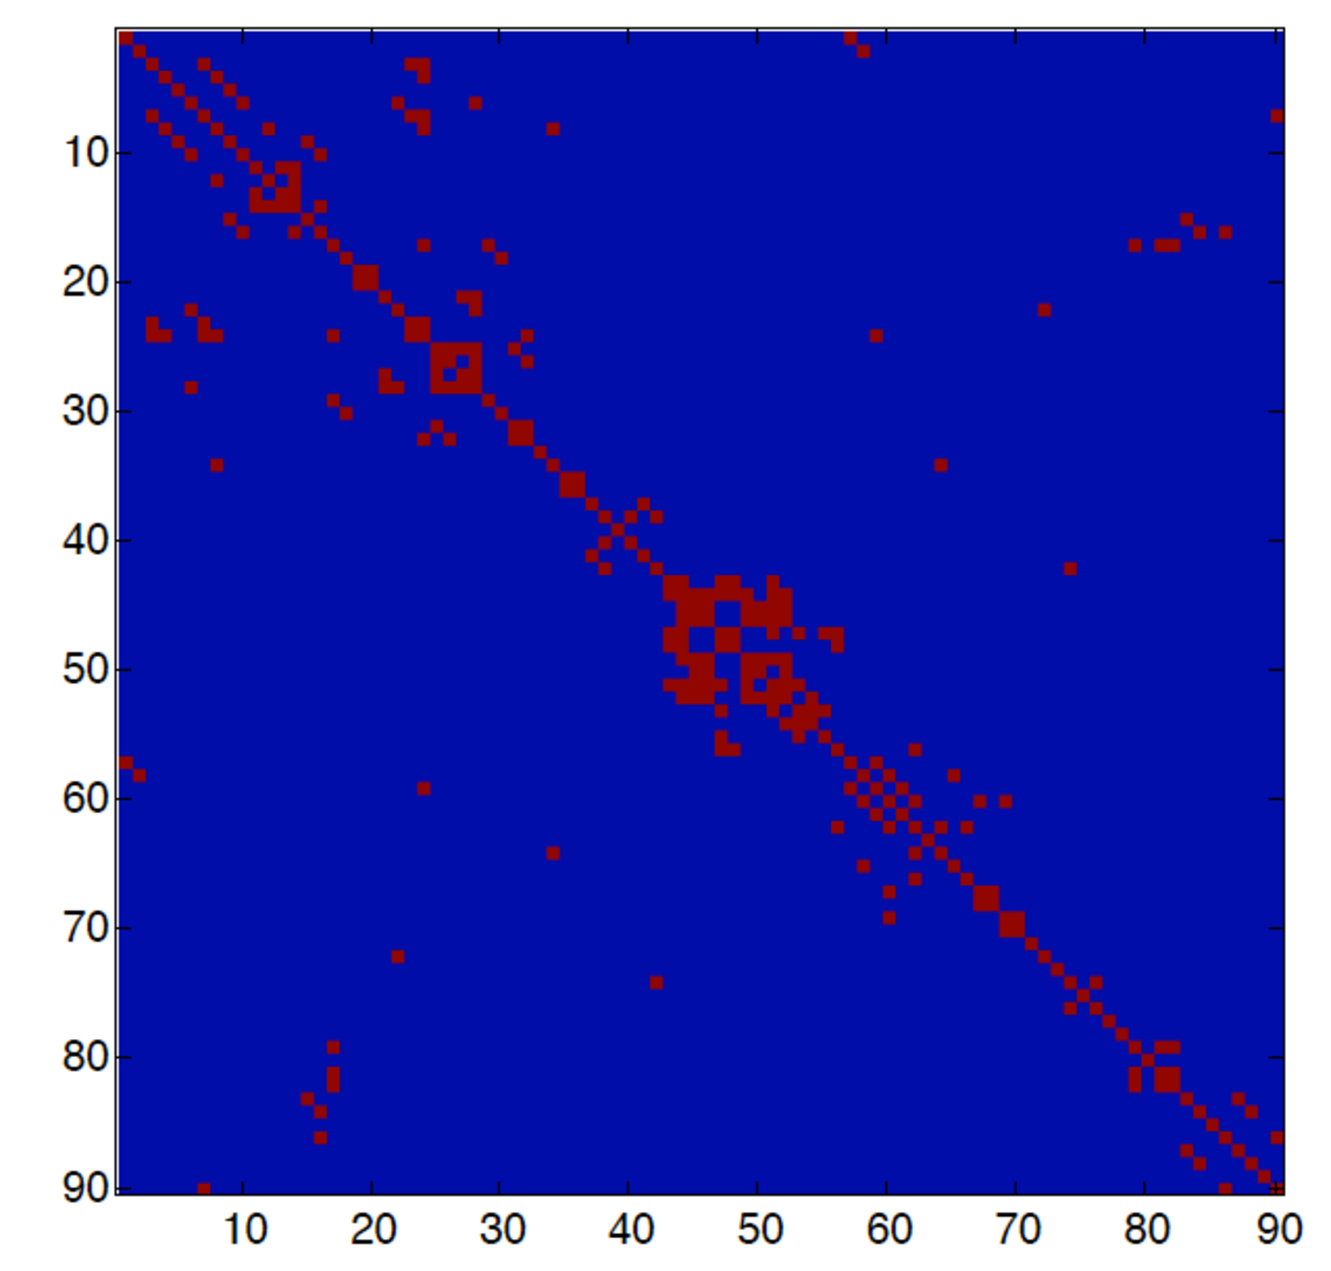
\includegraphics[width=0.515\textwidth,height=0.515\textheight,keepaspectratio]{figures/oldadjmatrix.pdf}
    }
    \caption{\small (a) Adjacency matrix in the young condition.   
  \small (b) Adjacency matrix old condition. The red dots prepresent connections between two nodes. The 
  number of edges in the young condition is 718 and in the young condition is 308, the average degree connectivity are 8.97 and 4.42 respectively.}
    \label{fig:adjmat}
  \end{figure} 
 
\subsection{Efficiency after single node lesioning}
\label{ss:single}
%2.perturbation analysis. Random random 1 node deletion
Here we build a population of networks created by the systematic lesioning of single nodes. 
The population of perturbations $P$ that result from the systematic deletion of all nodes in all possible combinations has as many networks as  
\begin{equation*}
|P| = \sum_{i=1}^{N} C(N,i) = \frac{N!} {(i!)(N-i)!}
\label{eq:perurb}
\end{equation*}

For example, the population of networks that result from the deletion of one single node has 90 networks 
\begin{equation*}
\sum_{i=1}^{1}
C(90,i) = \frac{90!} {(1!)(90-1)!} = 90
\end{equation*}

Similarly, the number of perturbed networks obtained by deleting two nodes in all possible ways contains 4005 networks
\begin{equation*}
\sum_{i=1}^{2} C(90,i)=
 \frac{90!} {(2!)(90-2)!} = 4005
\end{equation*}

We build a distribution of the efficiency measures described in section \ref{eq:latm}
for both young and elder condition for the systematic removal of one node. Thus, in the young condition, we denote $P_{y, 90}$ the distribution of networks with only one node removed, that is, $P_{y, 90}$ has 90 different networks where for each of of them, one node and its connections have been deleted. 
The mean of the efficiency measure for $P_{y, 90}$ is 0.358. The removal of node  "Inferior temporal gyrus" (89) has no effect in the efficiency, that is, the network efficiency before and after the removal has identical value. 
%Nodes 35 ("Median cingulate and paracingulate gyri") and 36 ("Posterior cingulate gyrus") have also an extremely mild effect after their removal. 
%deleted
%The fact that the PCC had nearly no effect on efficiency (interpreted as those regions having low connectivity degree) is inconsistent with previous work demonstrated that the PCC is one of the most structurally and functionally connected regions in the brain (for example, Crossley, Mechelli et al 2014, Brain). Why is this the case?
The most significant loss in efficiency occurs with the removal of node 74 ("Lenticular nucleus, putamen") followed by node 31 ("Insula right") . 
The average efficiency loss in the young condition is $2.44"\%" $ with a maximum of  $4.67"\%" $ for node 74 ("Lenticular nucleus, putamen") and no efficiency loss for node 89 ("temporal pole: middle temporal gyrus") (Figure \ref{fig:boxplot}). The rationale for the different impact in the efficiency caused by the obliteration of certain nodes can be found in the connectivity degree. In general, the nodes that after their removal trigger a low efficiency loss have also low connectivity degree, and those that produce a more pronounced reduction of the network efficiency tend to be more connected (Figure \ref{fig:gauss}, Figure \ref{fig:effloss}). 

Similarly, for the elder condition, we denote $P_{o, 90}$ the distribution of networks with only one node removed in the elder condition. 
The mean of the efficiency measure (equation \ref{eq:latm}) for the 90 networks obtained upon single node deletion is $0.109$. As it happened in the young condition, the removal of node 89 ("Temporal pole: middle temporal gyrus") has no effect in the efficiency. 
Interestingly, the removal of nodes with the lowest connectivity degree (2) have also no quantifiable effect in the network efficiency (Figure \ref{fig:boxplot}). 
%33,39,63,71,73,75,77,78,80,85 

The most significant loss in efficiency occurs with the removal of node node 62 ("Inferior parietal, but supramarginal and angular gyri"). After the removal of this node, the efficiency loss relative to the original network is the $32.87"\%"$. This is an interesting result since node 62 is not a highly connected node, its connectivity degree is 6. Nodes 24 ("Superior frontal gyrus, medial"), 44 ("Calcarine fissure and surrounding cortex") and 51 ("Middle occipital gyrus") have more connections, connectivity degree 10, and upon their deletion the efficiency loss is not as severe as in the case of node 62. 
The mean efficiency loss in the elder condition after the removal of a single node is  $4.61"\%"$. The effect in the loss of efficiency triggered by the disconnection of brain areas is more stereotypical i.e., less differentiated  in the elder condition than in young condition, that is, the connectivity degree alone is a much worse predictor of efficiency loss for old than for young subjects (Figure \ref{fig:gauss}, Figure \ref{fig:effloss}).
This is in agreement with the litterature of functional connectivity in healthy aging. The process of aging underlies global reorganization of brain functional networks that reflect the topological changes observed across the human lifespan \cite{cao_topological_2014}, \cite{song_age-related_2014}.  
Furthermore, as shown in \cite{geerligs_brain-wide_2015} brain networks in the elderly showed decreased modularity (less distinct functional networks) and decreased local efficiency.
%node 24, 0.2892 and the other 2 really small node 44 0.0387, node 51 0.0382

%Figure 2
\begin{figure}[!ht]
    \subfigure[Young: Network efficiency after one node deletion\label{subfig-1:dummy}]{%
      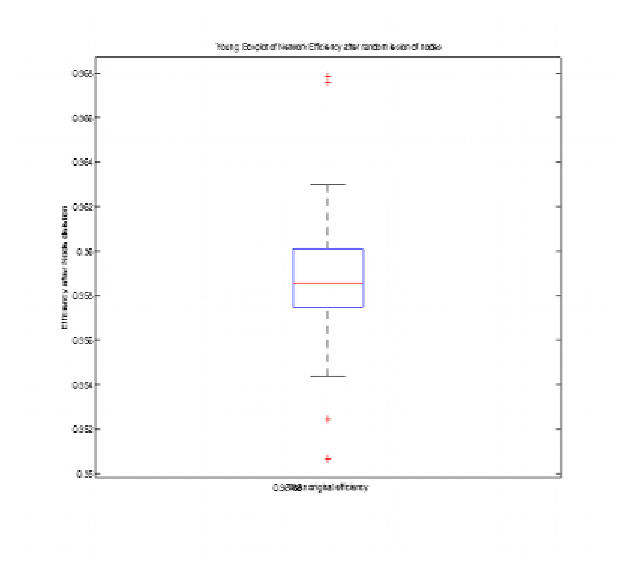
\includegraphics[width=0.49\textwidth]{figures/Fig-2-y-boxplot-eff_p.eps}
    }
    \hfill
    \subfigure[Old: Network efficiency after one node deletion\label{subfig-2:dummy}]{%
      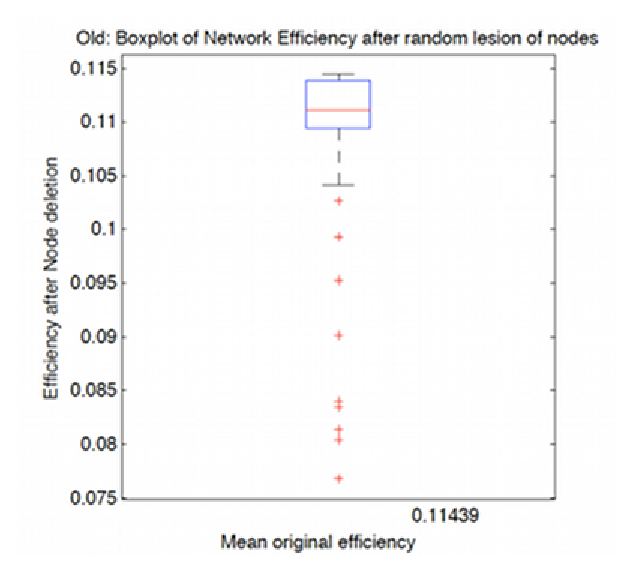
\includegraphics[width=0.46\textwidth]{figures/Fig-2-o-boxplot-eff_p.eps}
    }
     \subfigure[Young: Degree distribution (X) Efficiency loss (Y)\label{subfig-1:dummy}]{%
      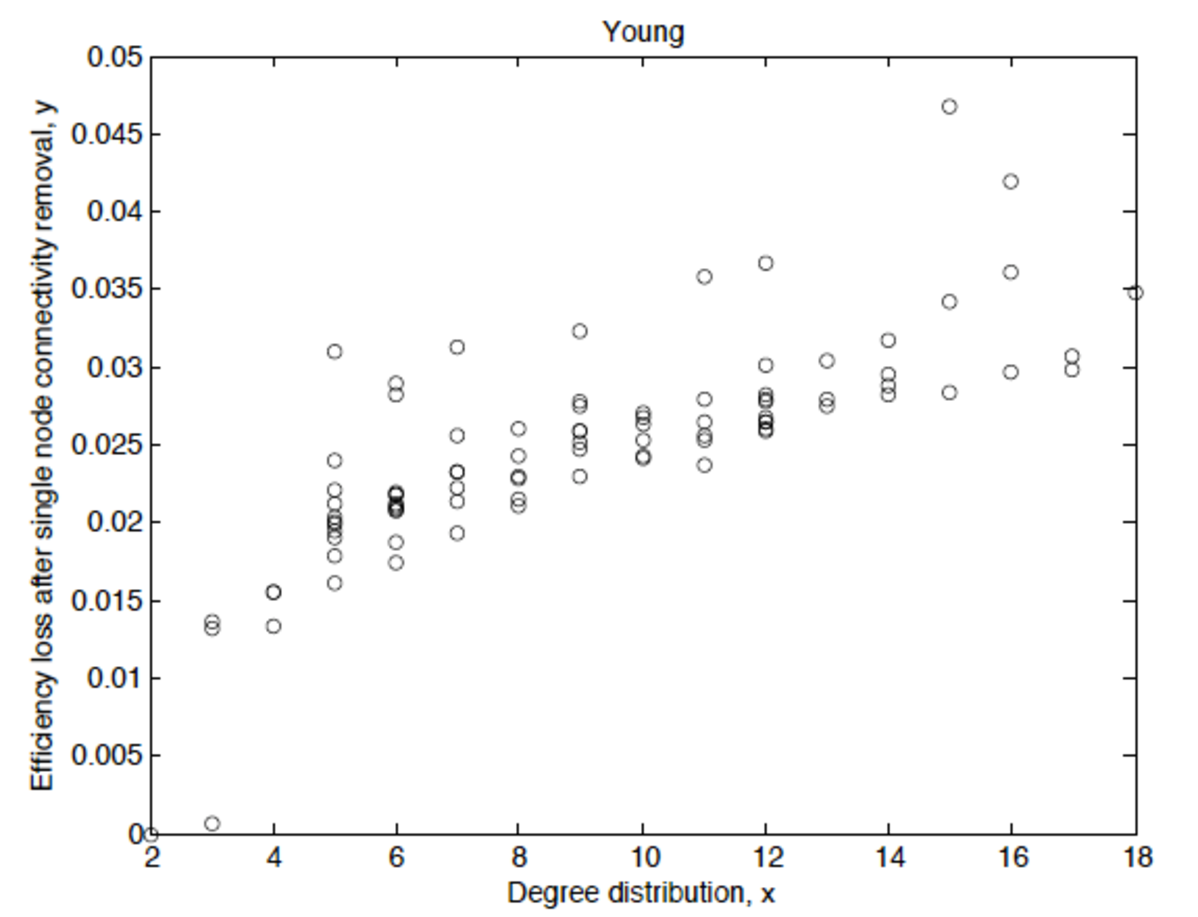
\includegraphics[width=0.49\textwidth]{figures/regressionyoung.pdf}
    }
    \hfill
    \subfigure[Old: Degree distribution (X) Efficiency loss (Y)\label{subfig-2:dummy}]{%
      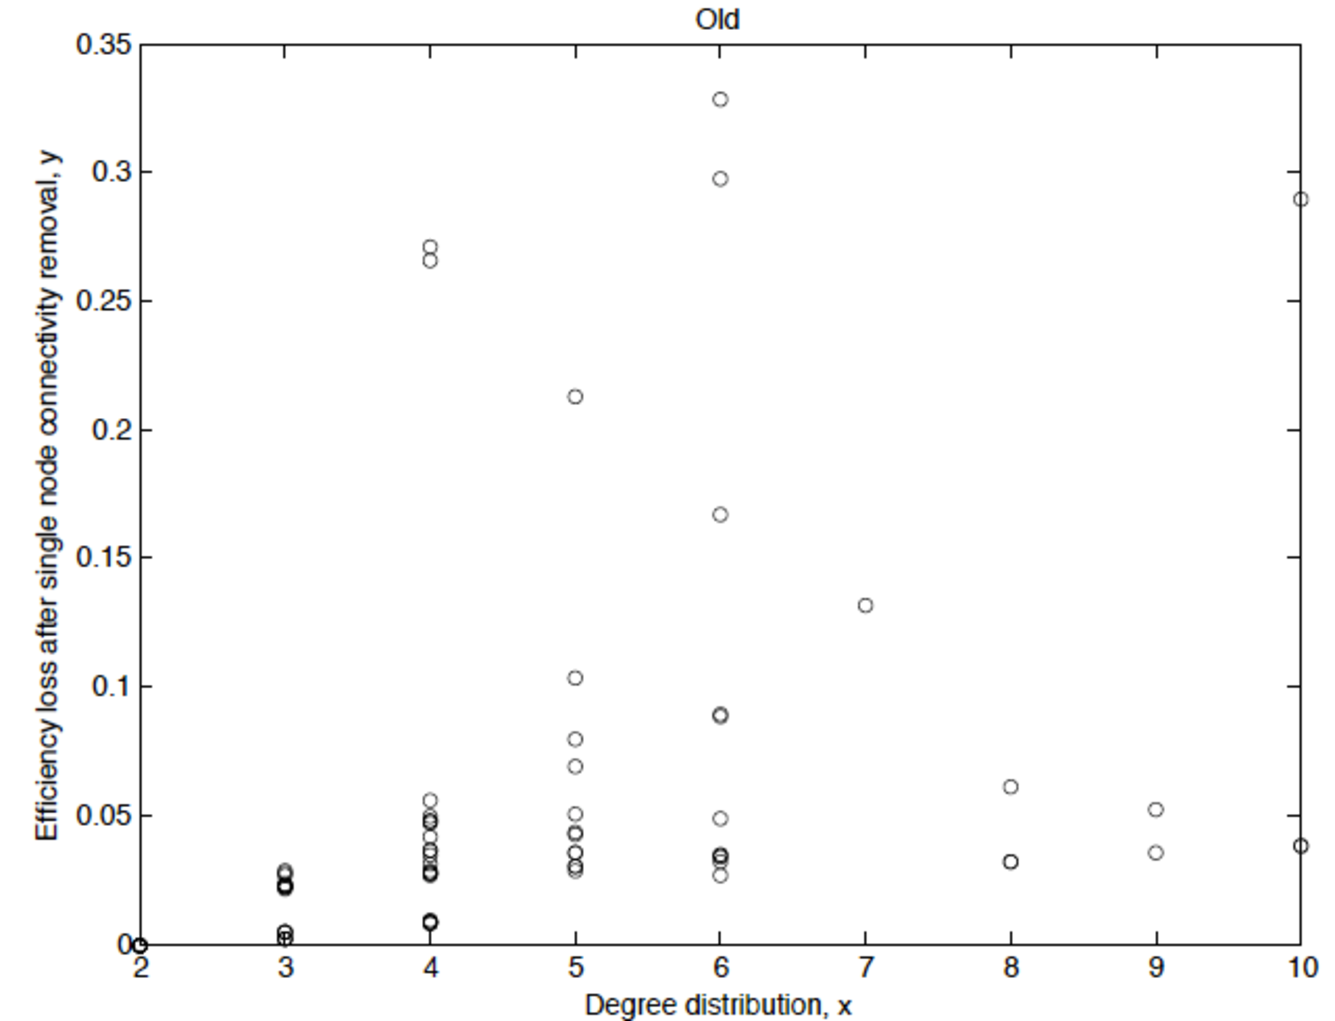
\includegraphics[width=0.48\textwidth]{figures/regressionold.pdf}
    }
    \caption{\small (a) Boxplot of network efficiency after random lesion of individual nodes. Only a very few nodes fall outside the box whose edges are the 25th and 75th percentiles. \small (b) Boxplot of network efficiency after random lesion of individual nodes. More nodes fall outside below the 25th percentile than in the young condition. The distribution in the elder condition is more skewed than in the young condition.\small (c) Degree distribution (x-axis) and efficiency loss or node centrality (y-axis) after single node connectivity removal in the young condition.  
  \small (d)  Degree distribution (x-axis) and efficiency loss node centrality (y-axis) after single node connectivity removal in the elder condition. Each dot in charts \small (c) and \small (d) represents a node with connectivity degree equals to x that upon its removal produces a variation in the network efficiency equals to y, normalized between 0 (no efficiency loss) and 1 (maximum efficiency loss). The linear regression in the young condition is 0.755 and in the old condition is 0.4002.}
    \label{fig:boxplot}
  \end{figure}

%Figure 3
\begin{figure}[!ht]
    \subfigure[Efficiency loss in young (blue) and old (red) for single node removal\label{subfig-1:dummy}]{%
      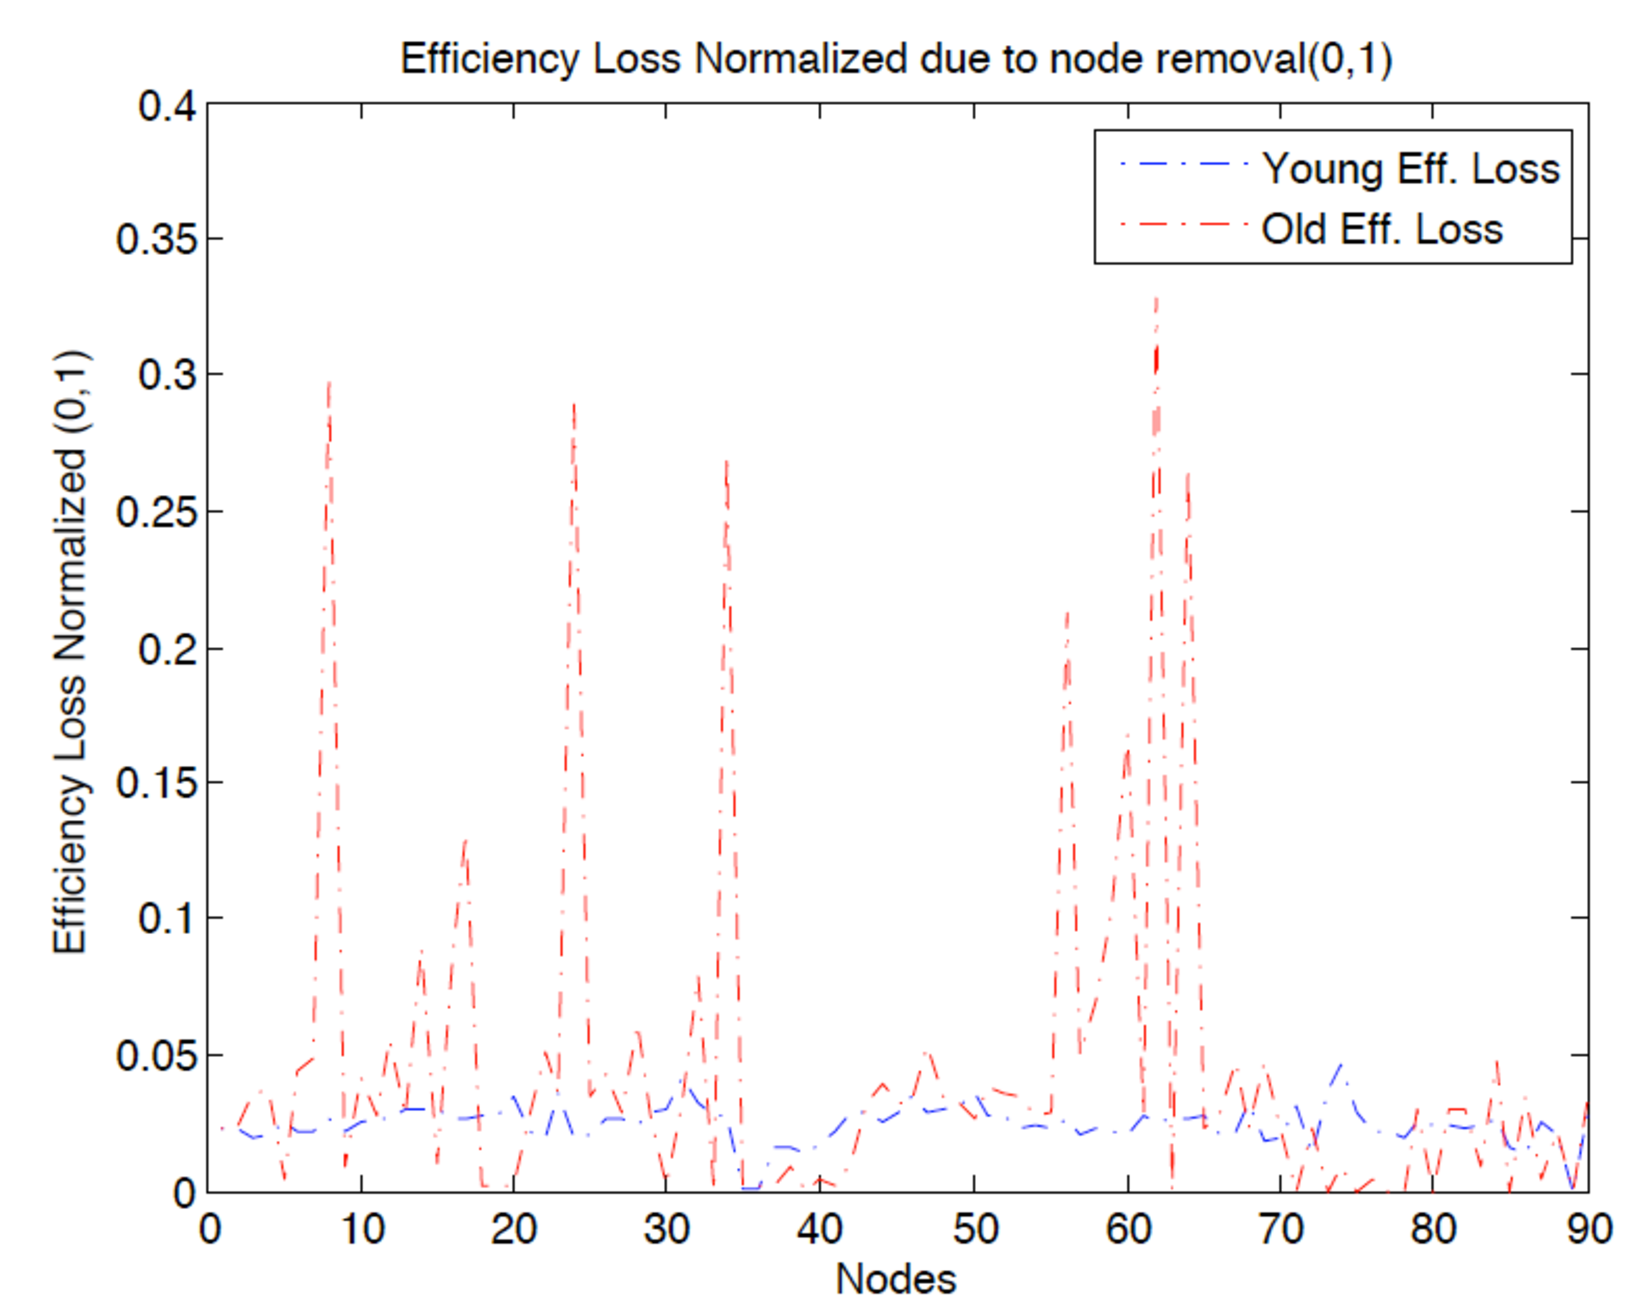
\includegraphics[width=0.51\textwidth,height=0.5\textheight,keepaspectratio]{figures/fig-4-eff-loss.pdf}
    }
    \hfill
    \subfigure[Frequency bars for efficiency loss in young (green) and old (blue) for single node removal\label{subfig-2:dummy}]{%
      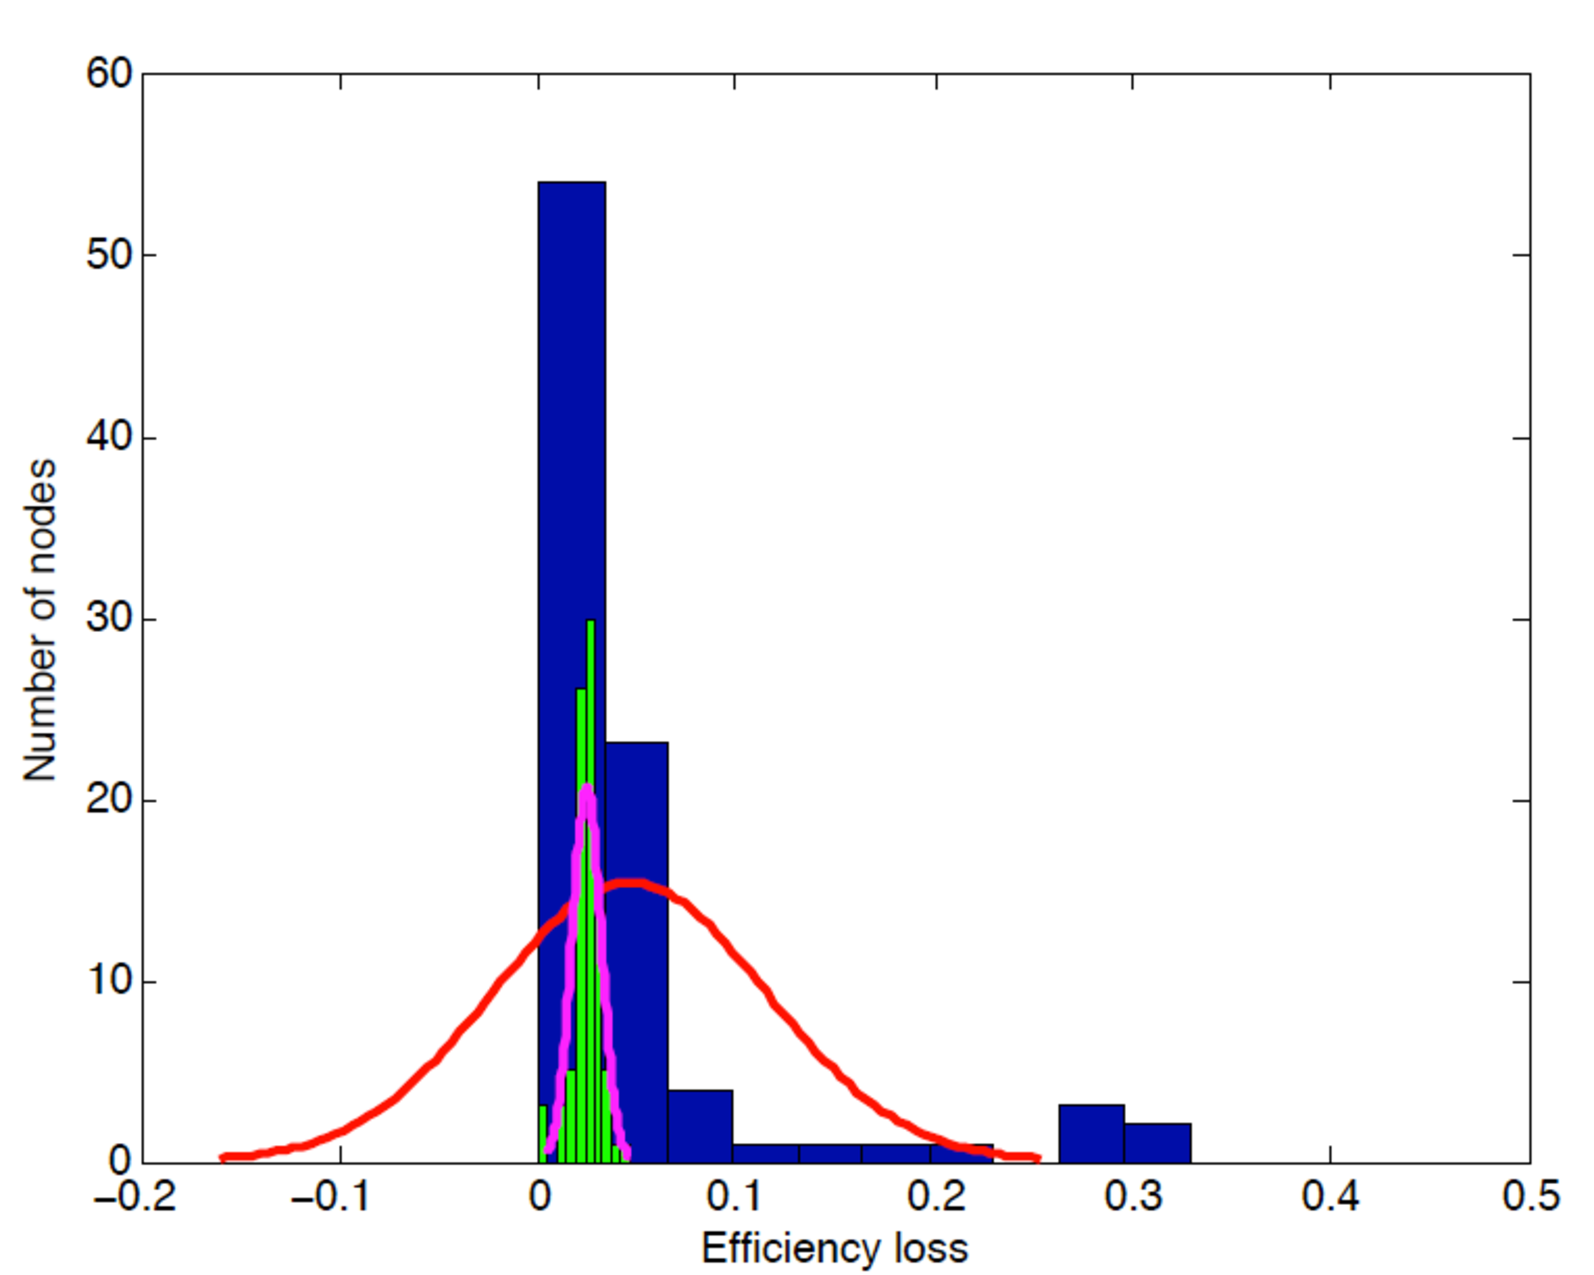
\includegraphics[width=0.5\textwidth,height=0.5\textheight,keepaspectratio]{figures/lossdistrib-greenisYoung-blueisold.pdf}
    }     
    \caption{\small (a) Efficiency loss normalized (0,1) due to the removal of each node in both elder and young condition. While in the young condition there are no nodes that upon its removal the efficiency of the resulting network deteriorates drastically, in the elder condition, there are 6 nodes that upon their removal trigger a $20\%$ or more reduction in the network efficiency. Nodes 8 ("Middle frontal gyrus"), $29.7\%$  24 ("Superior frontal gyrus, medial"), $28.9\%$   34 ("Median cingulate and paracingulate gyri"), $27.1\%$  56 ("Fusiform gyrus"),$21.2\%$  62 ("Inferior parietal, but supramarginal and angular gyri"), $32.8\%$  and 64 ("Supramarginal gyrus"), $26.5\%$ of efficiency loss.   
  \small (b) Distribution of efficiency loss after node removal in both young (green histogram) and elder condition (blue histogram). The efficiency loss in the young condition is narrow. The elder condition, on the other hand, has a more spread distribution of efficiency values. 
The range in efficiency loss in the young condition varies a $4.67\%$ and in the elder condition varies a $32.87\%$}
    \label{fig:gauss}
  \end{figure} 

\begin{figure}[H]
    \subfigure[Efficiency loss in young subjects\label{subfig-1:dummy}]{%
      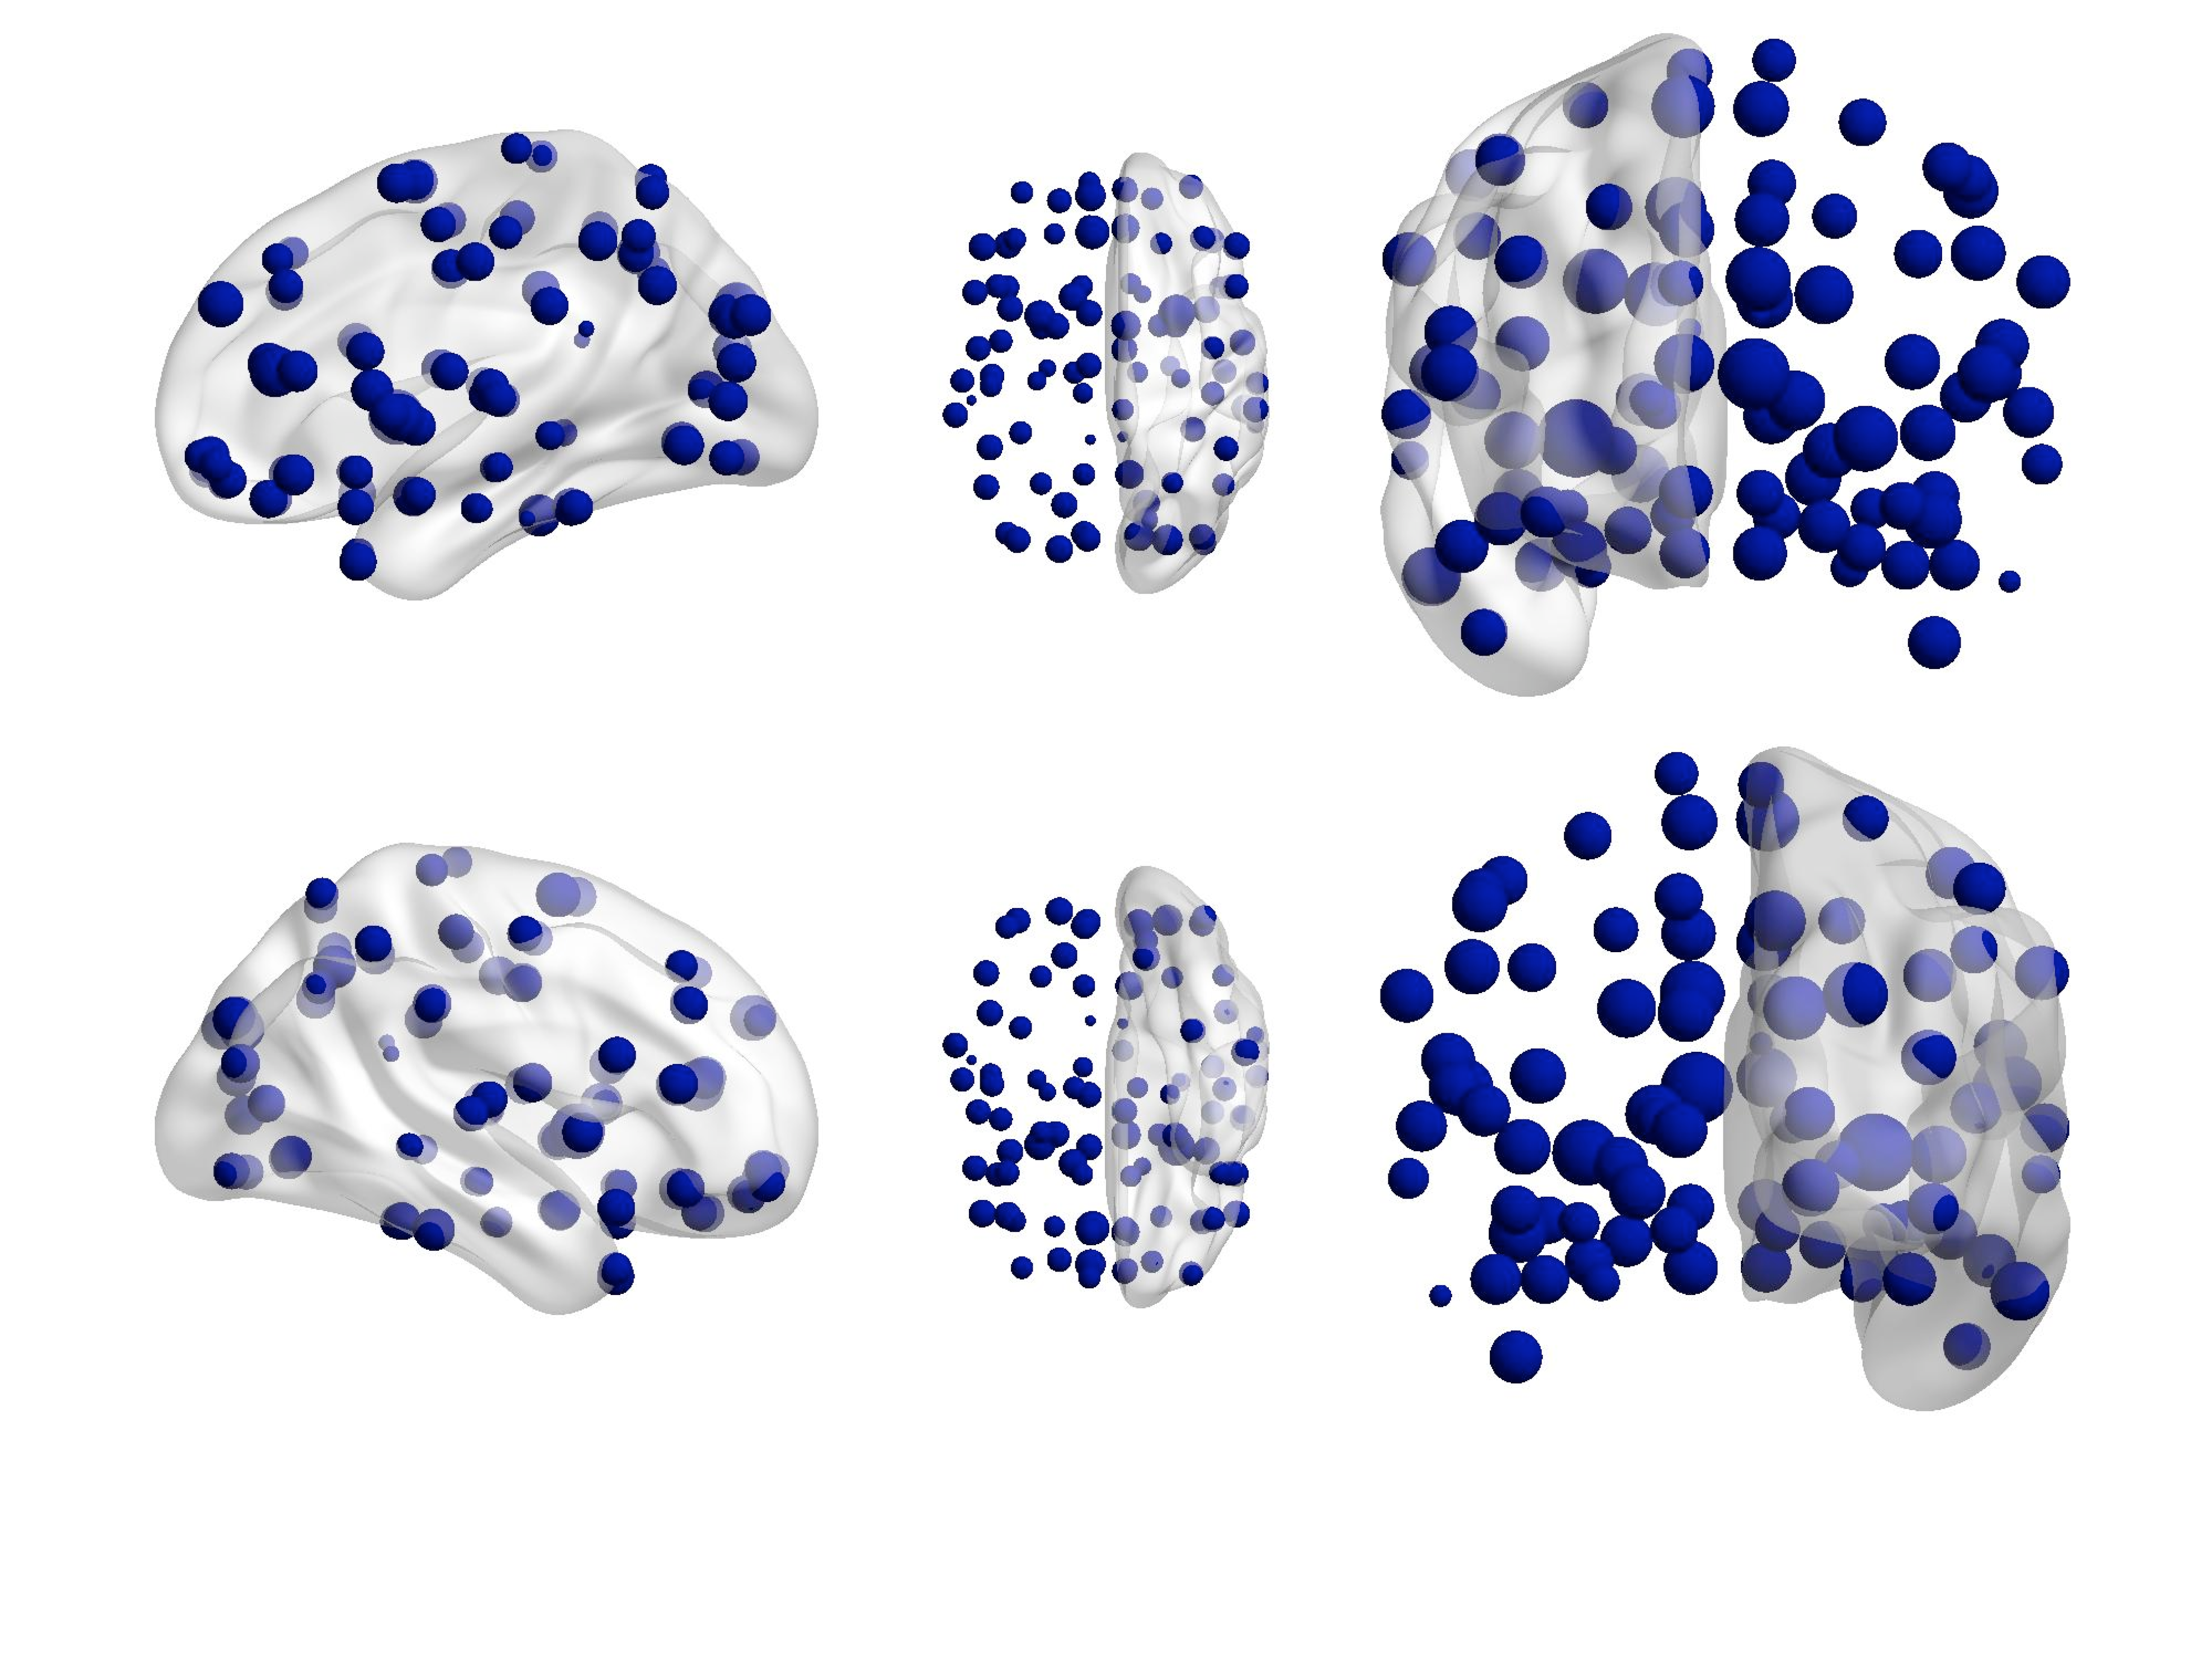
\includegraphics[width=0.5\textwidth,height=0.5\textheight,keepaspectratio]{figures/Young_Nodes_Full_EffLossx100.pdf}
    }
    \hfill
    \subfigure[Efficiency loss in old subjects\label{subfig-2:dummy}]{%
      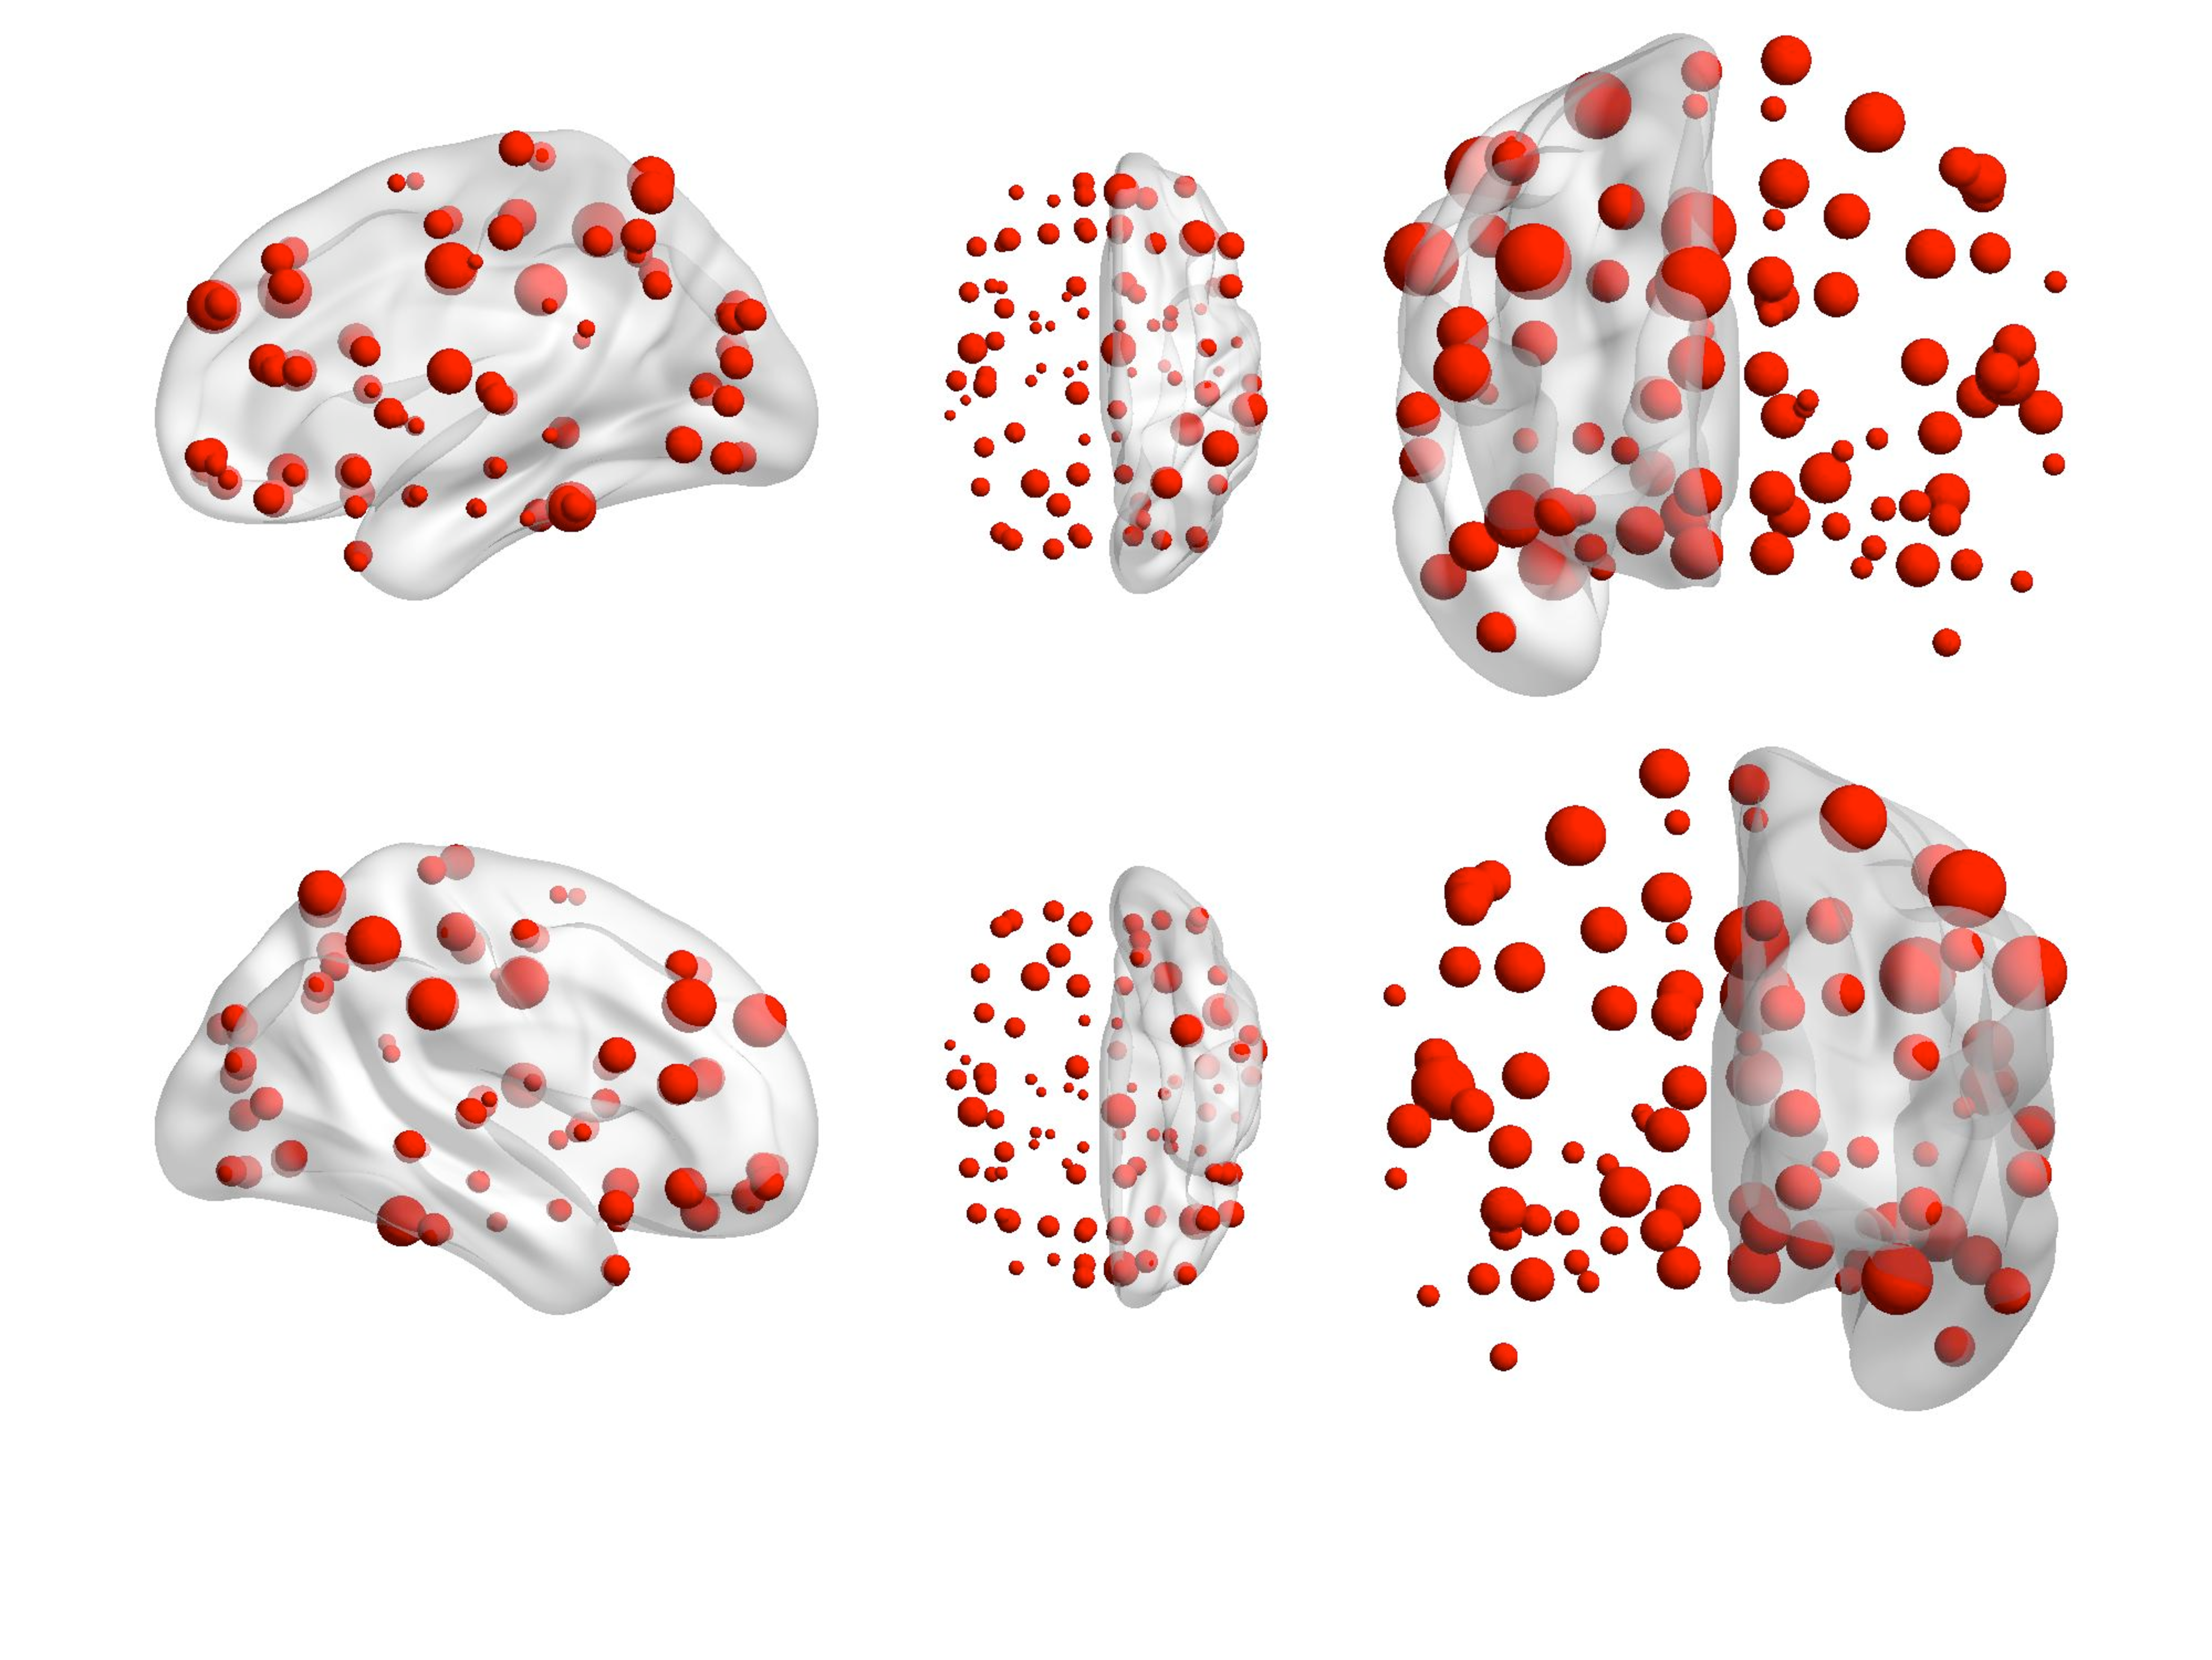
\includegraphics[width=0.5\textwidth,height=0.5\textheight,keepaspectratio]{figures/Old_Nodes_Full_EffLossx100.pdf}
    }     
    \caption{Efficiency loss in young and elder condition for single node removal. The larger the dot size, the larger is the efficiency loss upon its removal.} 
    %\small (a) Efficiency loss in young (blue)  \small (b) Efficiency loss in old (red).}
    \label{fig:effloss}
  \end{figure} 


\subsection{Efficiency after target networks lesioning}
\label{ss:target}
So far, we have quantified the efficiency loss due to the removal of single nodes, in this section we investigate how the efficiency measure is affected by the removal of entire networks of interest. In particular, we study the efficiency loss of eight different brain networks, namely, the Default Mode Network (DMN), temporal lobe, frontal lobe, insula and cingulate gyrus, occipital lobe, parietal lobe, central structures and limbic structures (Figure \ref{fig:targetbn}).
 
%%Hypothesis testing
The DMN is commonly considered to consist of medial prefrontal cortex
(AAL 23, 24, 25, 26), posterior cingulate cortex/precuneus (AAL 35, 36/67 68)
and bilateral inferior parietal lobule (AAL 61, 62). 
The removal of the DMN in
young adults triggers an efficiency loss of the $19.6\%$. In the elder condition, the same procedure yields an efficiency reduction of $61.66\%$. It is remarkable that in the elder condition the lesioning of the DMN network, which represents the $11\%$ of the total regions 90 regions, bring down the efficiency of the network to $61.66\%$.
%Figure DMN
The strong efficiency reduction associated with the lesioning of the DMN in old subjects is coherent with the hypothesis that there is a decrease in activity in the DMN in aging \cite{koch_effects_2010}. This age-based reduction in DMN activity can trigger mechanisms that compensate the loss in DMN activity with an increase in connectivity between the DMN and other networks \cite{damoiseaux_reduced_2008}. According to this hypothesis, the DMN becomes a more central network and upon the lesioning of the DMN a dramatic efficiency loss is produced. 

%- "The older subjects exhibited significantly lower DMN activity in the posterior cingulate (PCC, t-test P<.001) as well as a tendency to lower activity in all other DMN regions in comparison to the younger subjects. TEST this: We found no significant effect of age on DMN inter-connectivity."
%http://www.ncbi.nlm.nih.gov/pubmed/20004726

%http://www.ncbi.nlm.nih.gov/pmc/articles/PMC4392680/
%The vision-related brain regions (hereafter called Visual) in the AAL template include left and right calcarine fissure and surrounding cortex (Nodes 45,46), left and right lingual gyrus (Nodes 47,49), left and right superior occipital gyrus (Nodes 49,50), left and right middle occipital gyrus (Nodes 51, 52), left and right inferior occipital gyrus (Nodes 53, 54), left and right fusiform gyrus (Nodes 55, 56), left and right superior parietal gyrus (Nodes 59,60), and right inferior temporal gyrus (Nodes 89, 90). The removal of the Visual network in young adults triggers an efficiency loss of the $38.93\%$ while in the elder condition the same procedure yields a $55.98\%$. 
The removal of the frontal lobe, the parietal lobe and the temporal lobe have as well a larger impact in the elder condition than in the young condition. 
Interestingly, we have identified three brain networks in which the lesioning in young individuals has a larger impact compared to old subjects. The lesioning of the occipital lobe trigger a slightly lower efficiency loss value in the old condition compared to the young condition. More interestingly is the lesioning of the limbic structures and the central structures. The efficiency loss for these structures shows a distinct diference between young and old individuals with larger values for the former. The minor impact of the lesioning of central and limbic structures in the old condition is conforming with the literature that shows degradation of fronto-stratial network in aging \cite{salami_elevated_2014} and the break-down between the hipocampal regions and the DMN \cite{fjell_brain_2015}. 

%The degradation of fronto-striatal network in task studies has been suggested to be a driving force of memory decline in aging. The connectivity of fronto-striatal pathways are also related to self-esteem \cite{fjell_brain_2015}. The removal of fronto-striatal edges in the young condition the removal of edges that connect the frontalstratium pathways gives a reduction of efficiency of $0.37\%$. In the old condition, there are no  edges connecting fronto-stratial areas and therefore there is no efficiency loss associated to this lesioning.  
%Frontostriatal circuits are neural pathways that connect frontal lobe regions with the basal ganglia (striatum) that mediate motor, cognitive, and behavioural functions within the brain. 
\begin{figure}[!ht]
    \caption{Connectivity network for target network removal in both conditions.}%(Table \ref{tab:nodesn}) }

    \subfigure[DMN lesioning in young\label{subfig-1:dummy}]{%
      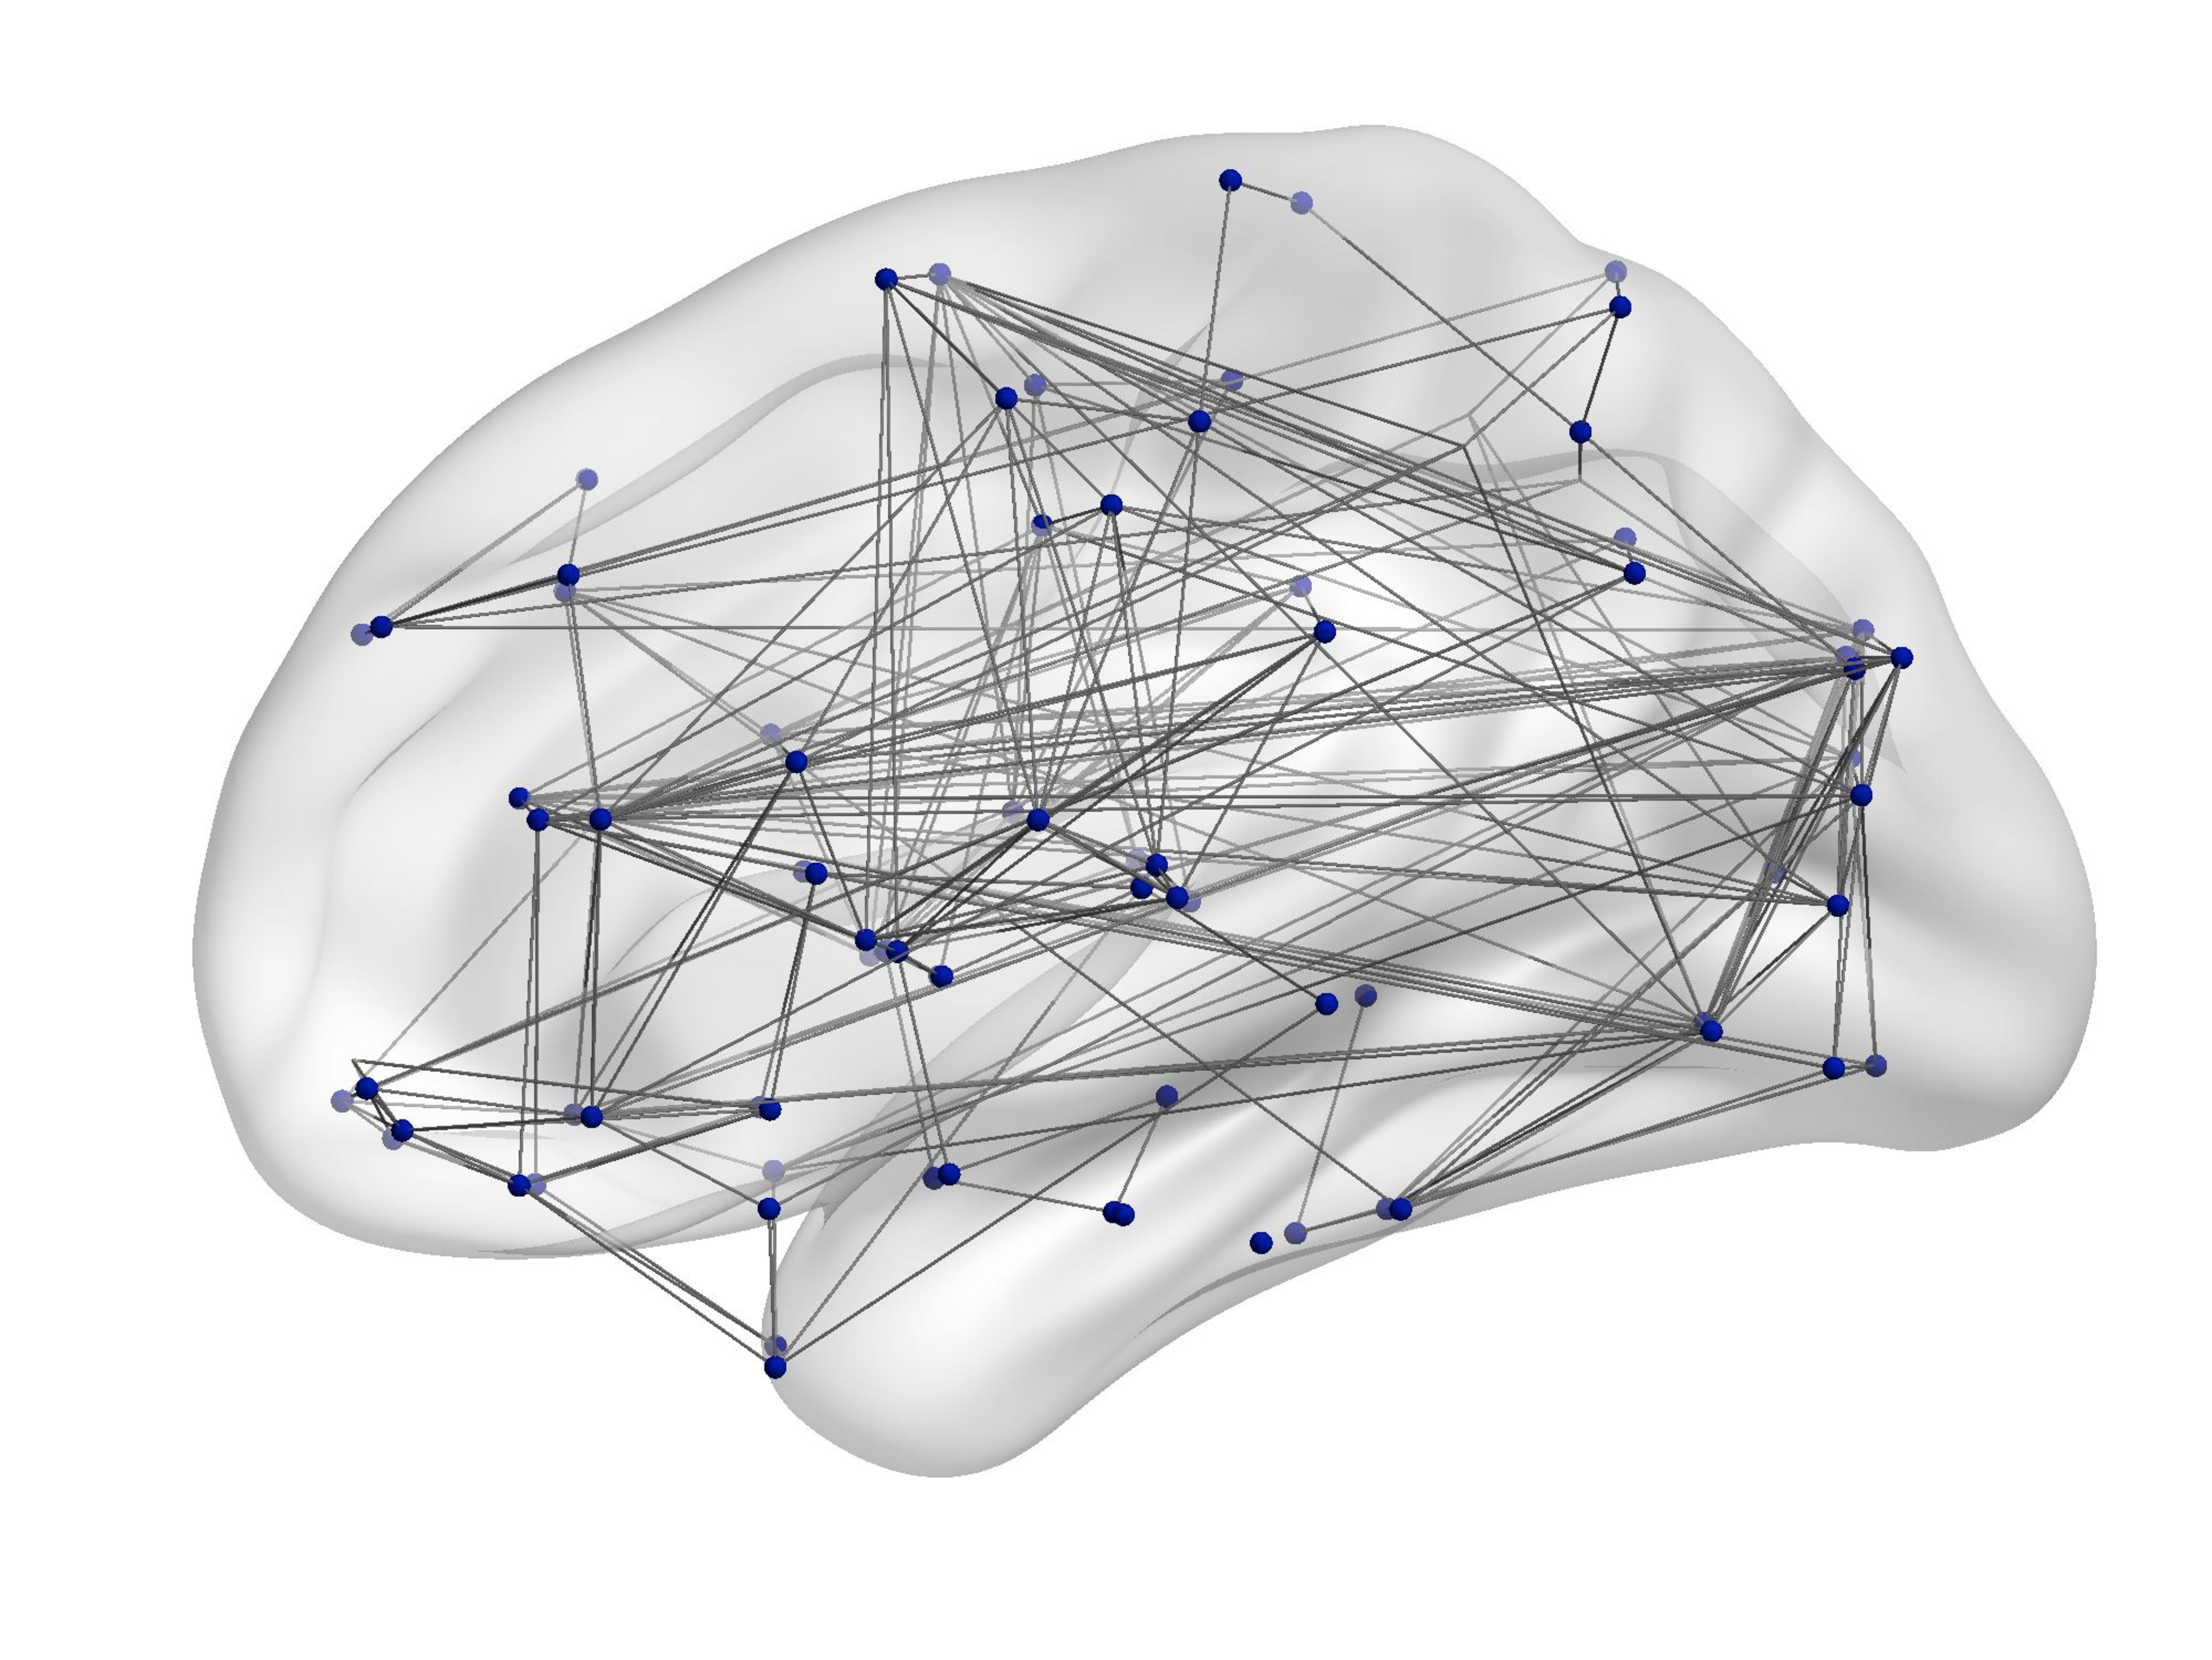
\includegraphics[width=0.4\textwidth,height=0.2\textheight,keepaspectratio]{figures/Young-DMN-Sagittal.pdf}
    }
\subfigure[DMN lesioning in elderly \label{subfig-2:dummy}]{%
      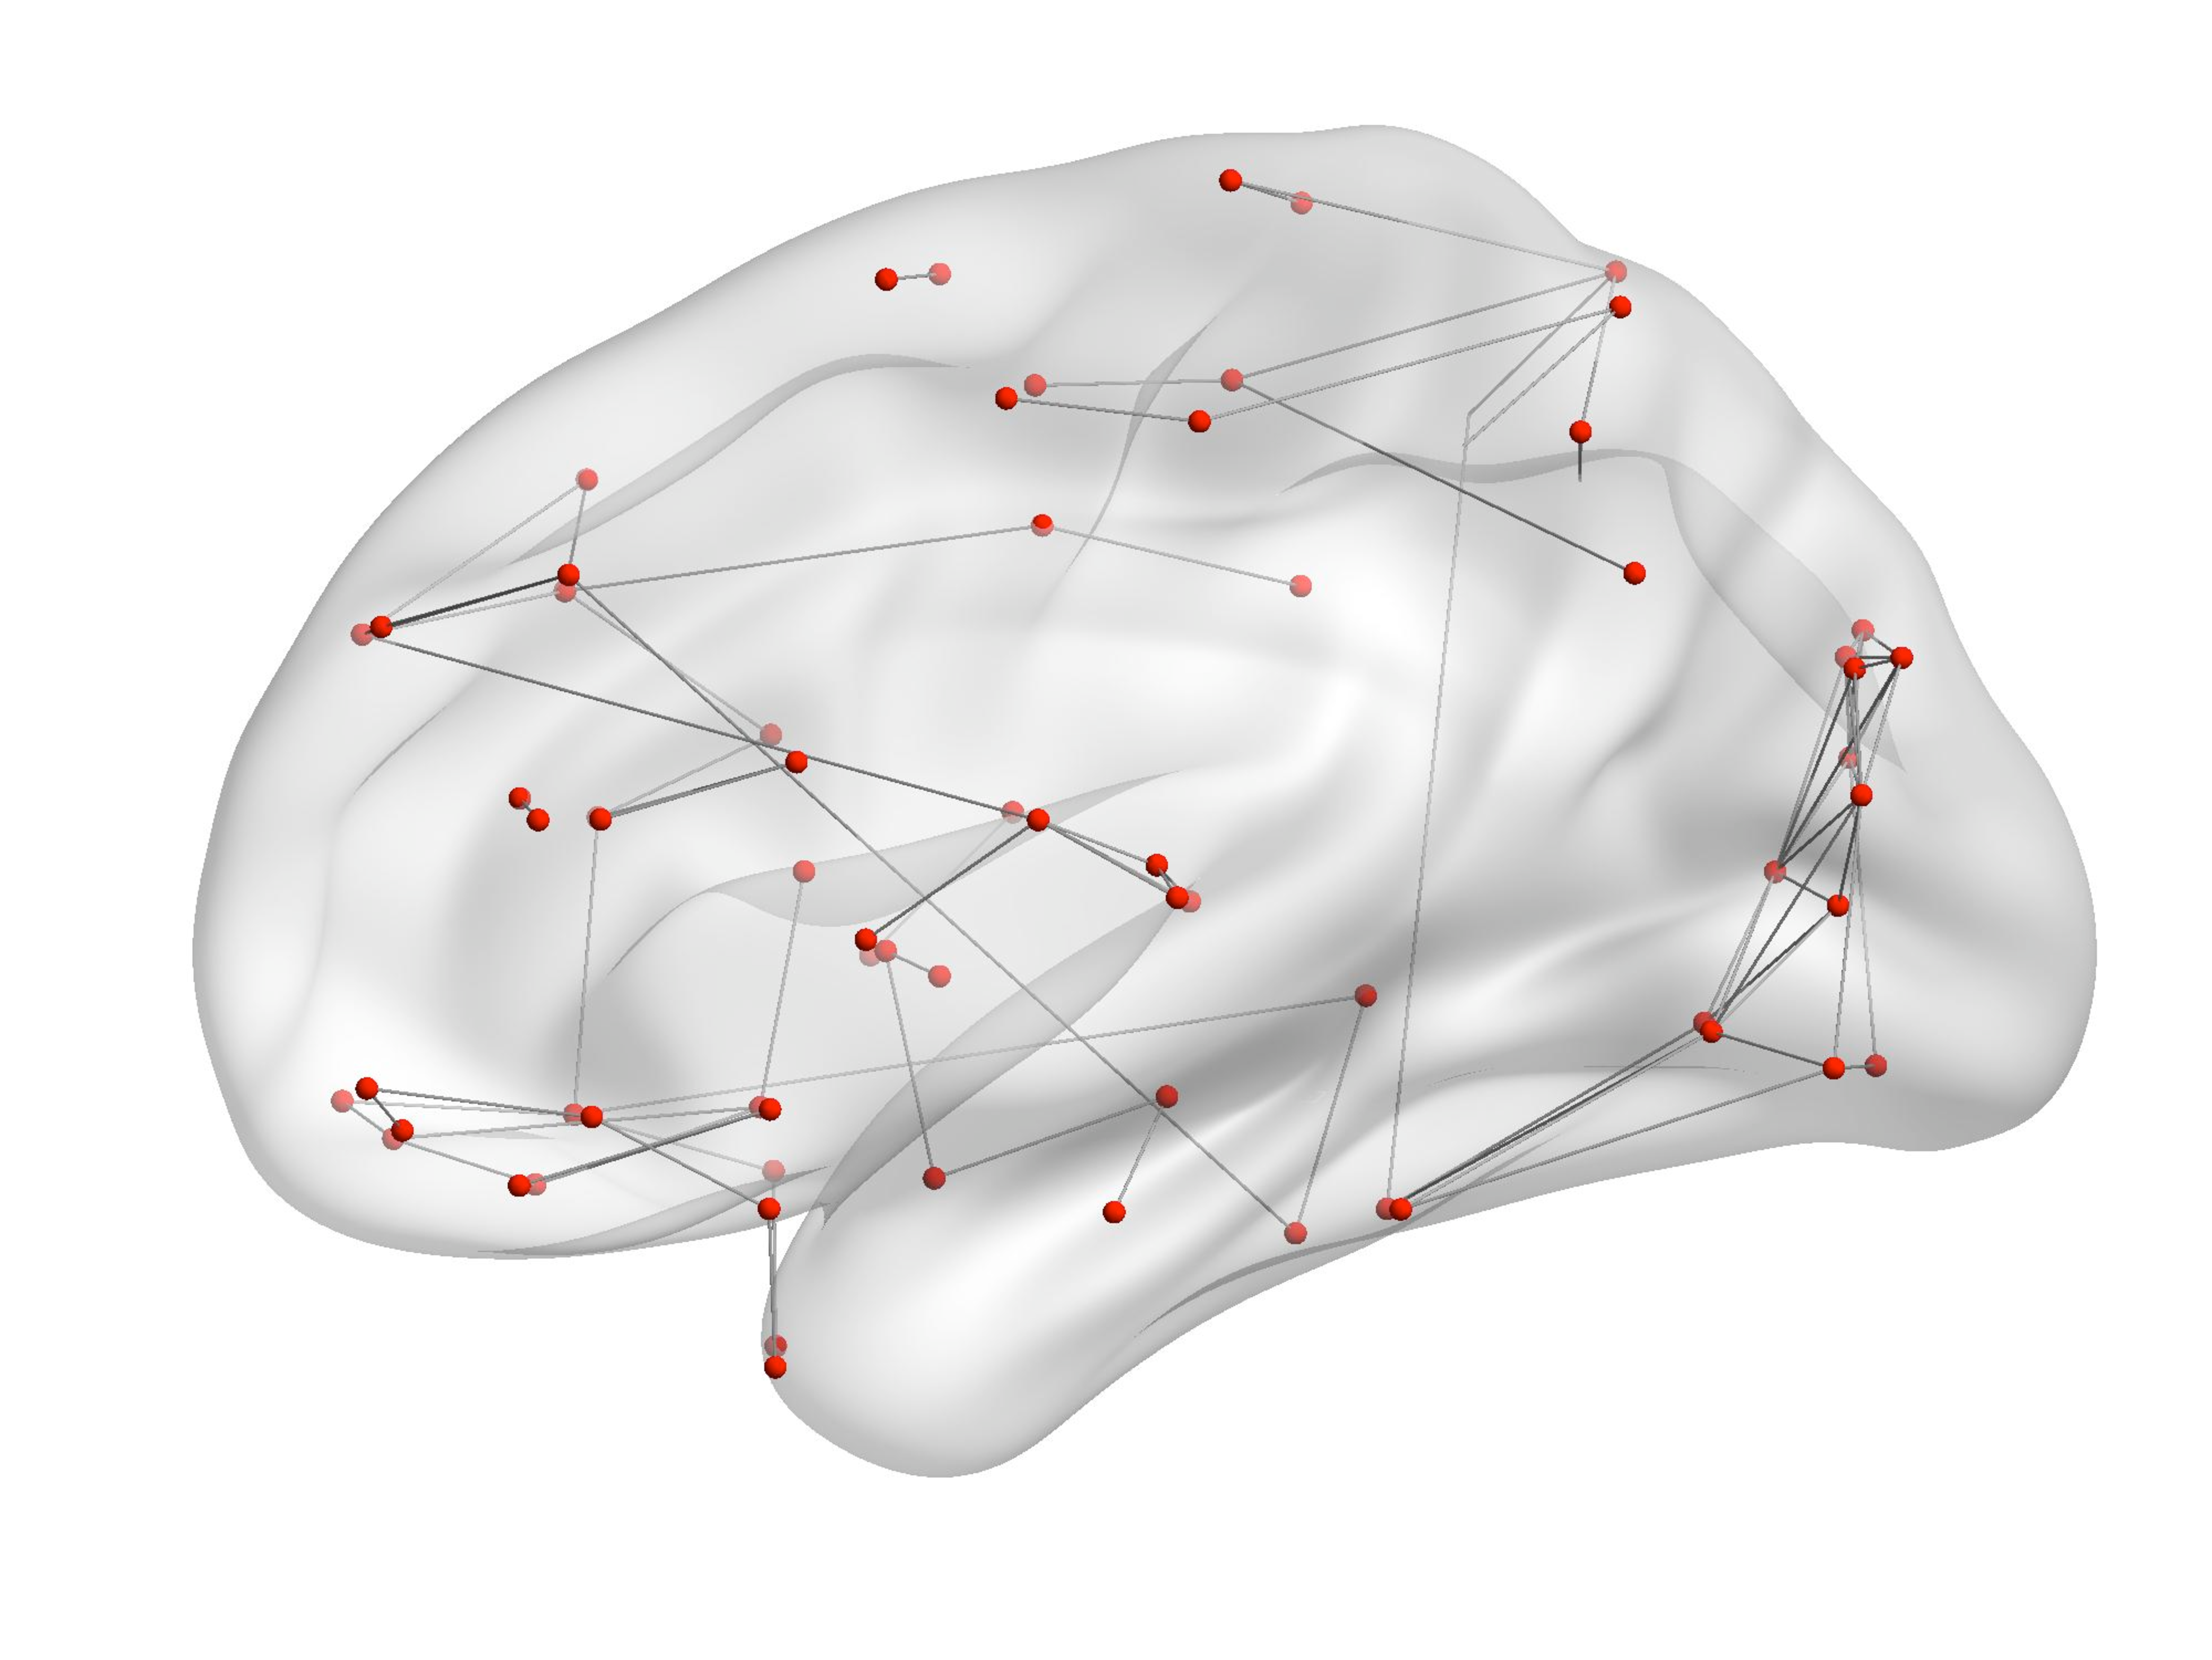
\includegraphics[width=0.4\textwidth,height=0.2\textheight,keepaspectratio]{figures/Old-DMN-Sagittal.pdf}
    }    
     \hfill
    \subfigure[Frontal lesioning in young\label{subfig-1:dummy}]{%
      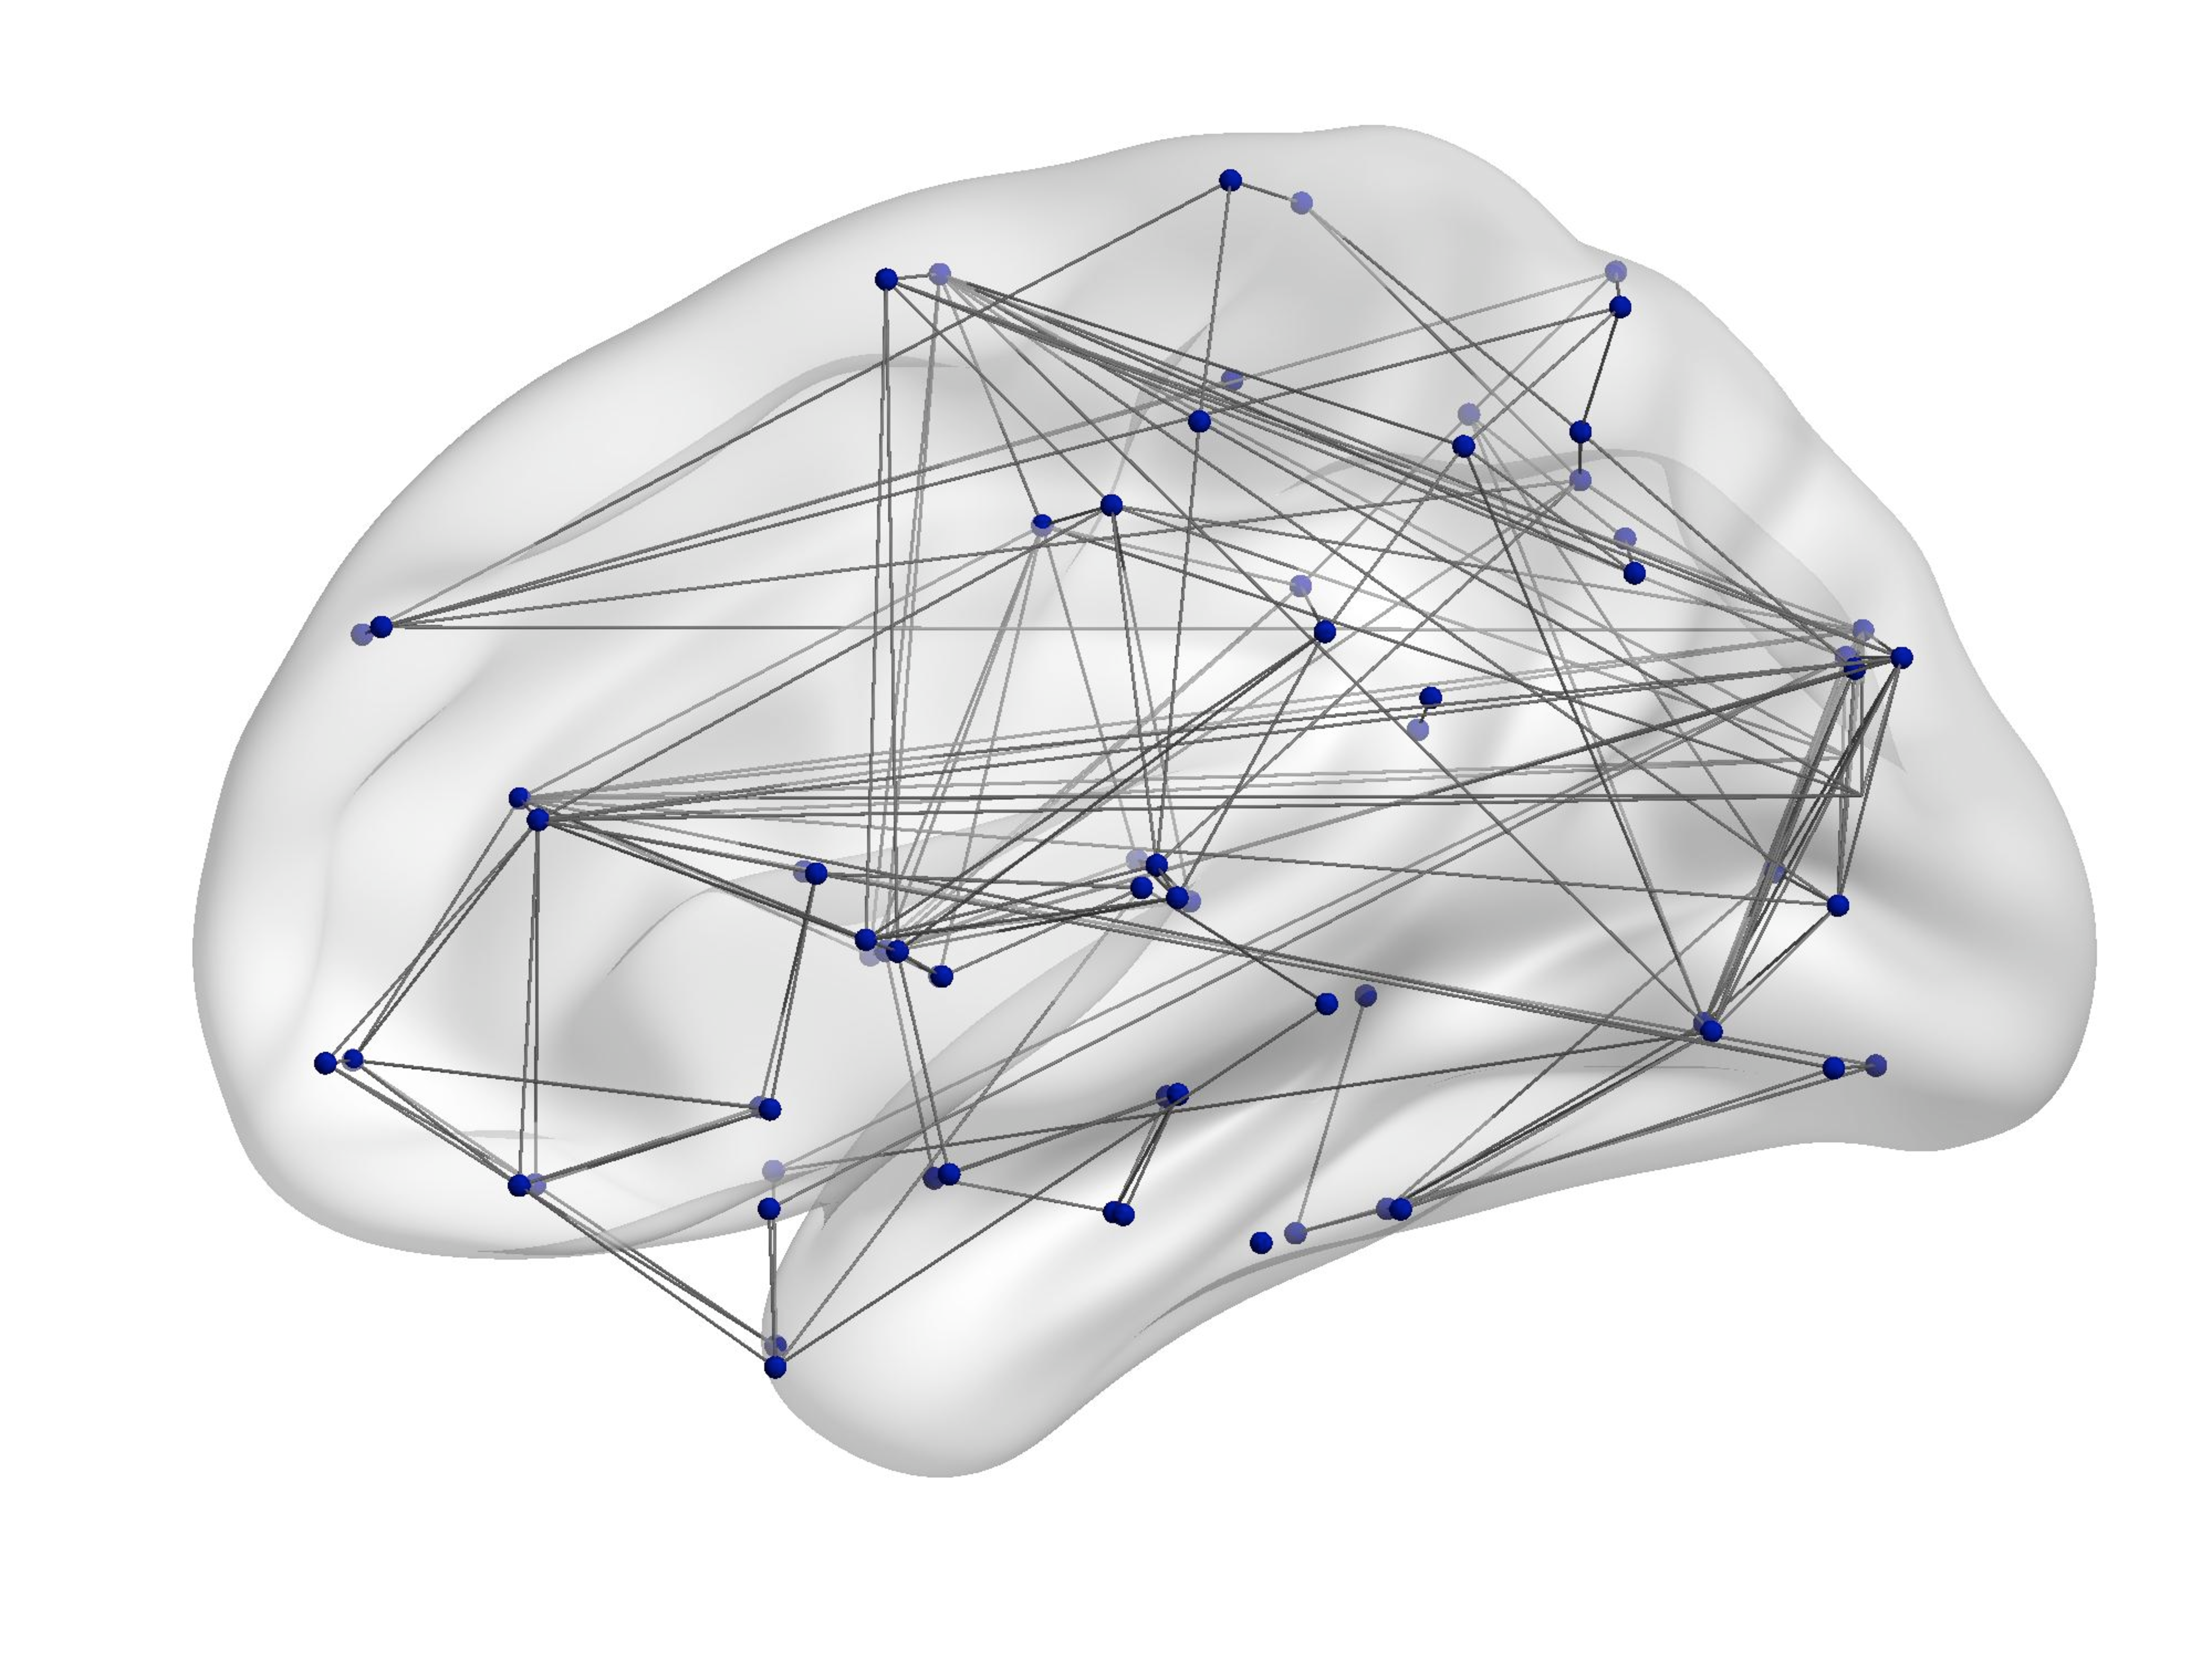
\includegraphics[width=0.4\textwidth,height=0.2\textheight,keepaspectratio]{figures/Young-Frontal-Sagittal.pdf}
    }
 \hfill
    \subfigure[Limbic lesioning in elderly\label{subfig-2:dummy}]{%
      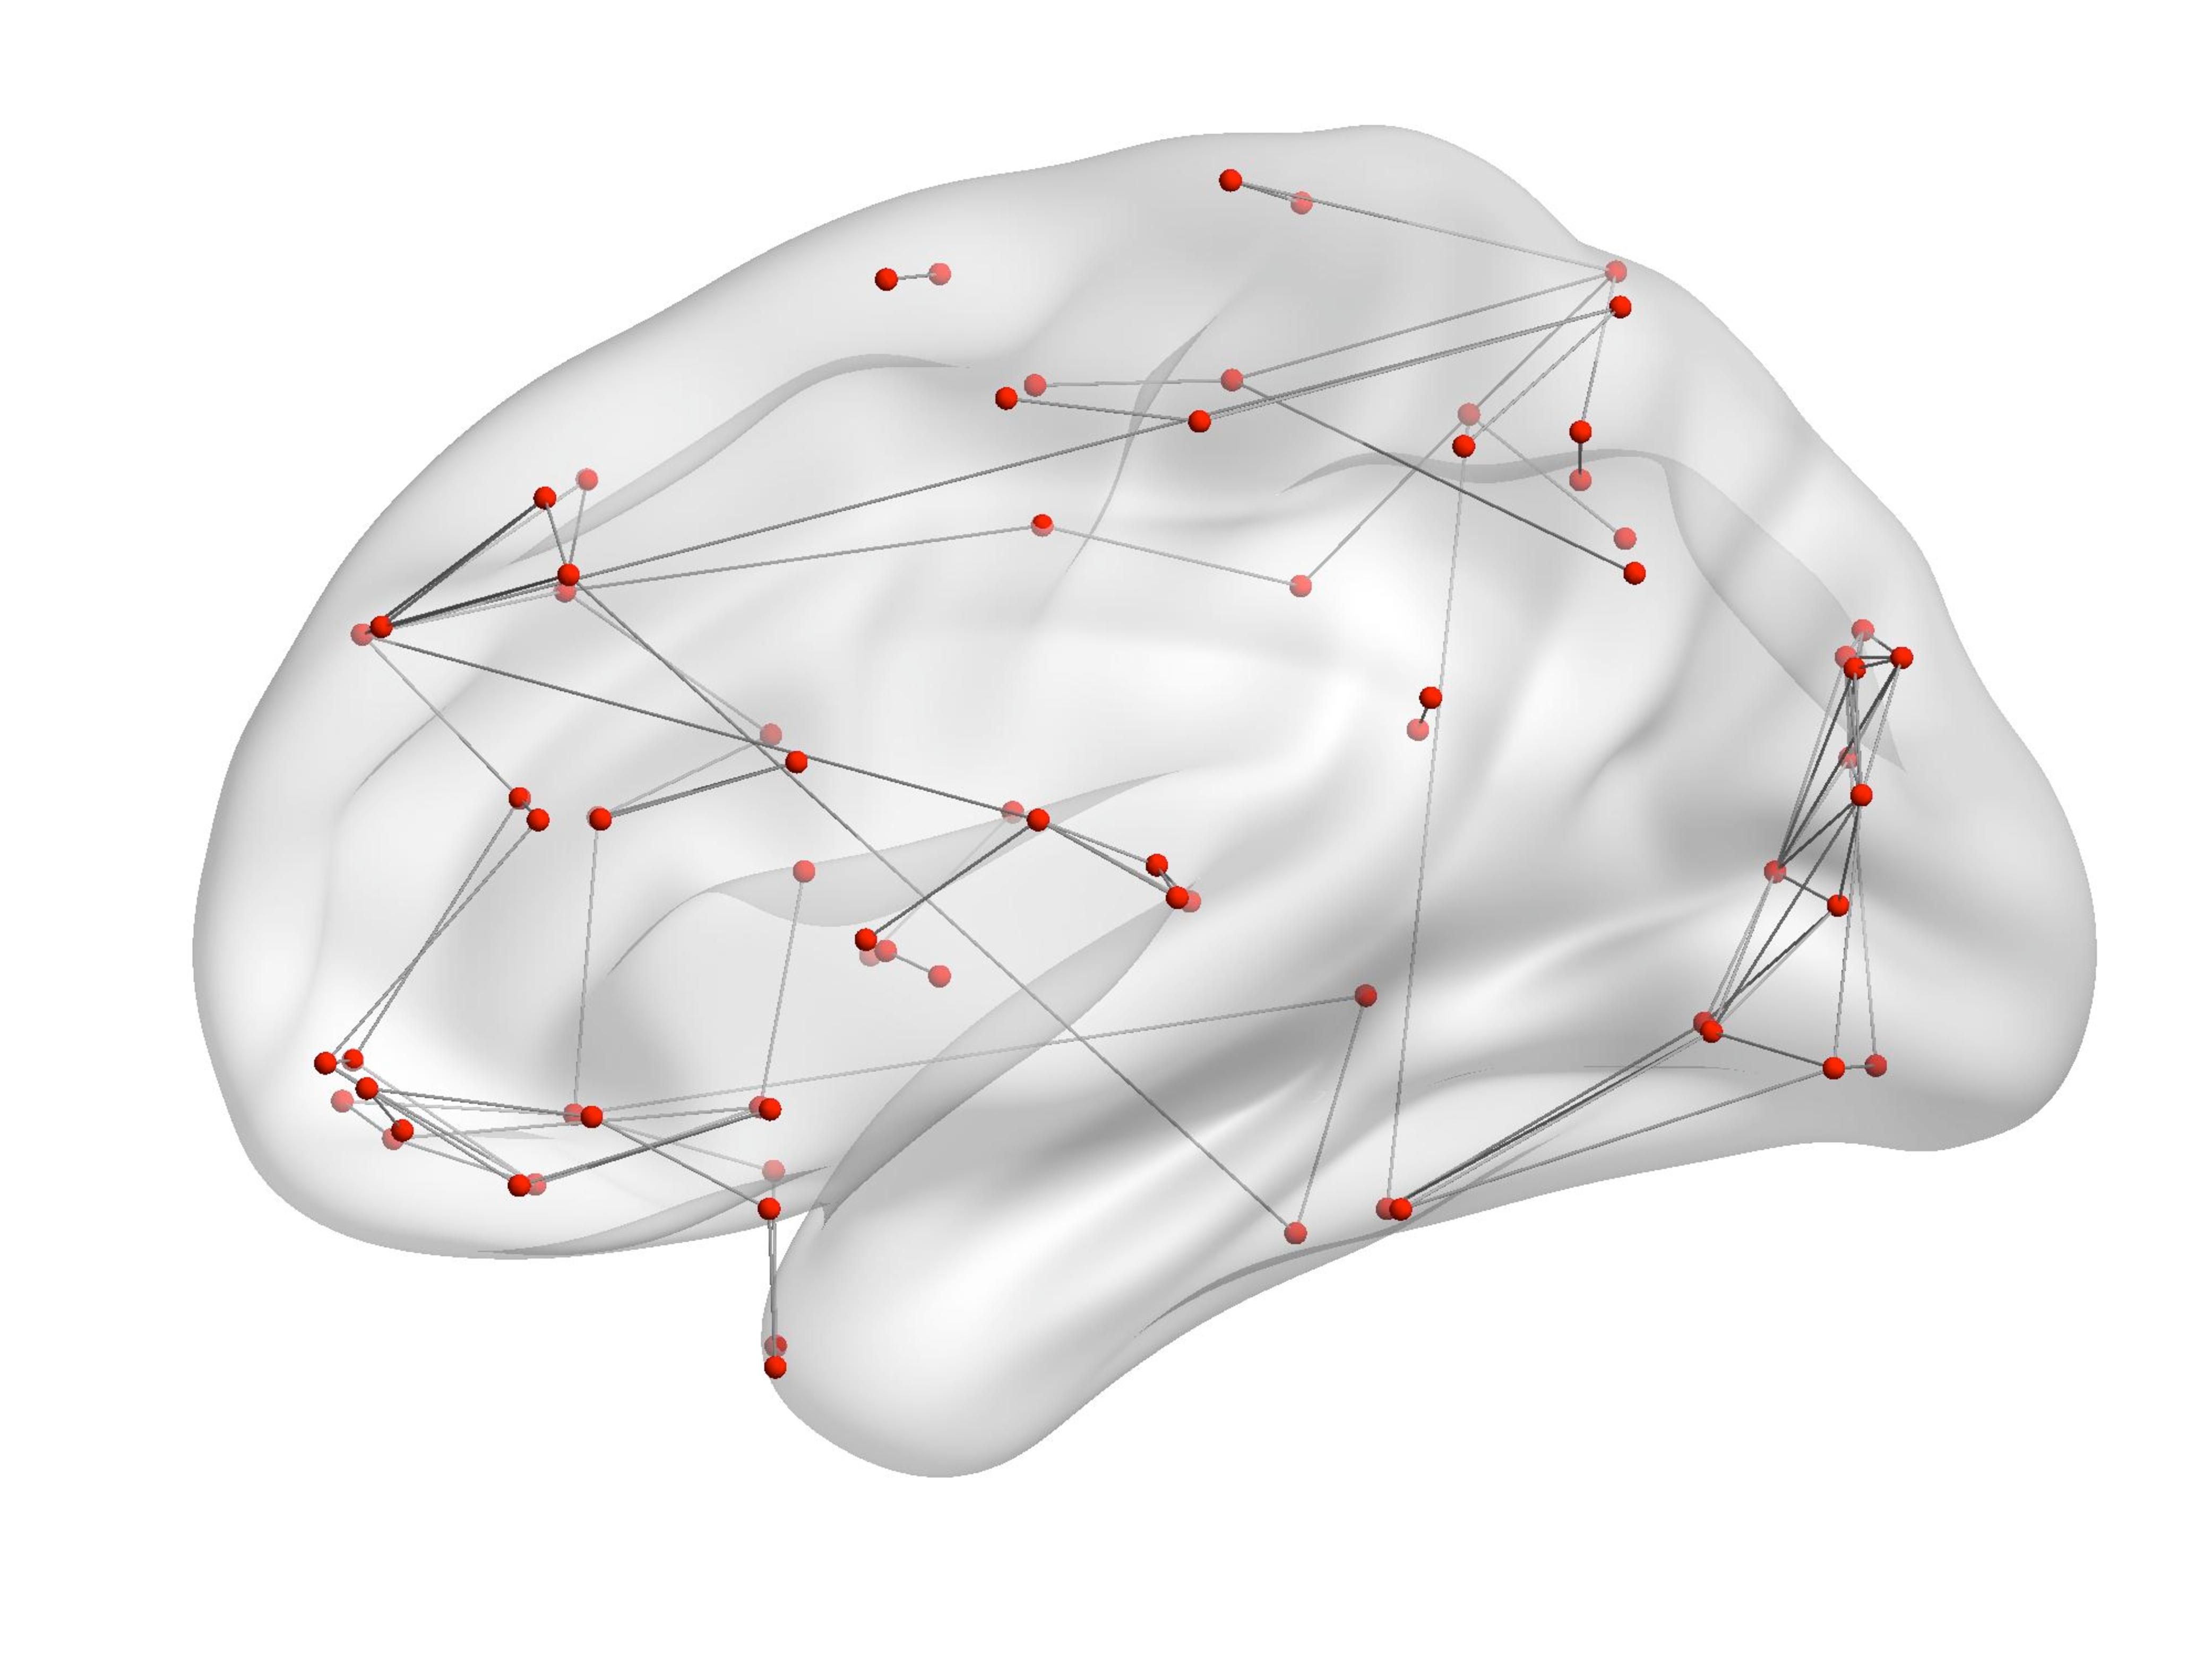
\includegraphics[width=0.4\textwidth,height=0.2\textheight,keepaspectratio]{figures/Old-Limbic-Sagittal.pdf}
    }   
    \subfigure[Central lesioning in young \label{subfig-1:dummy}]{%
      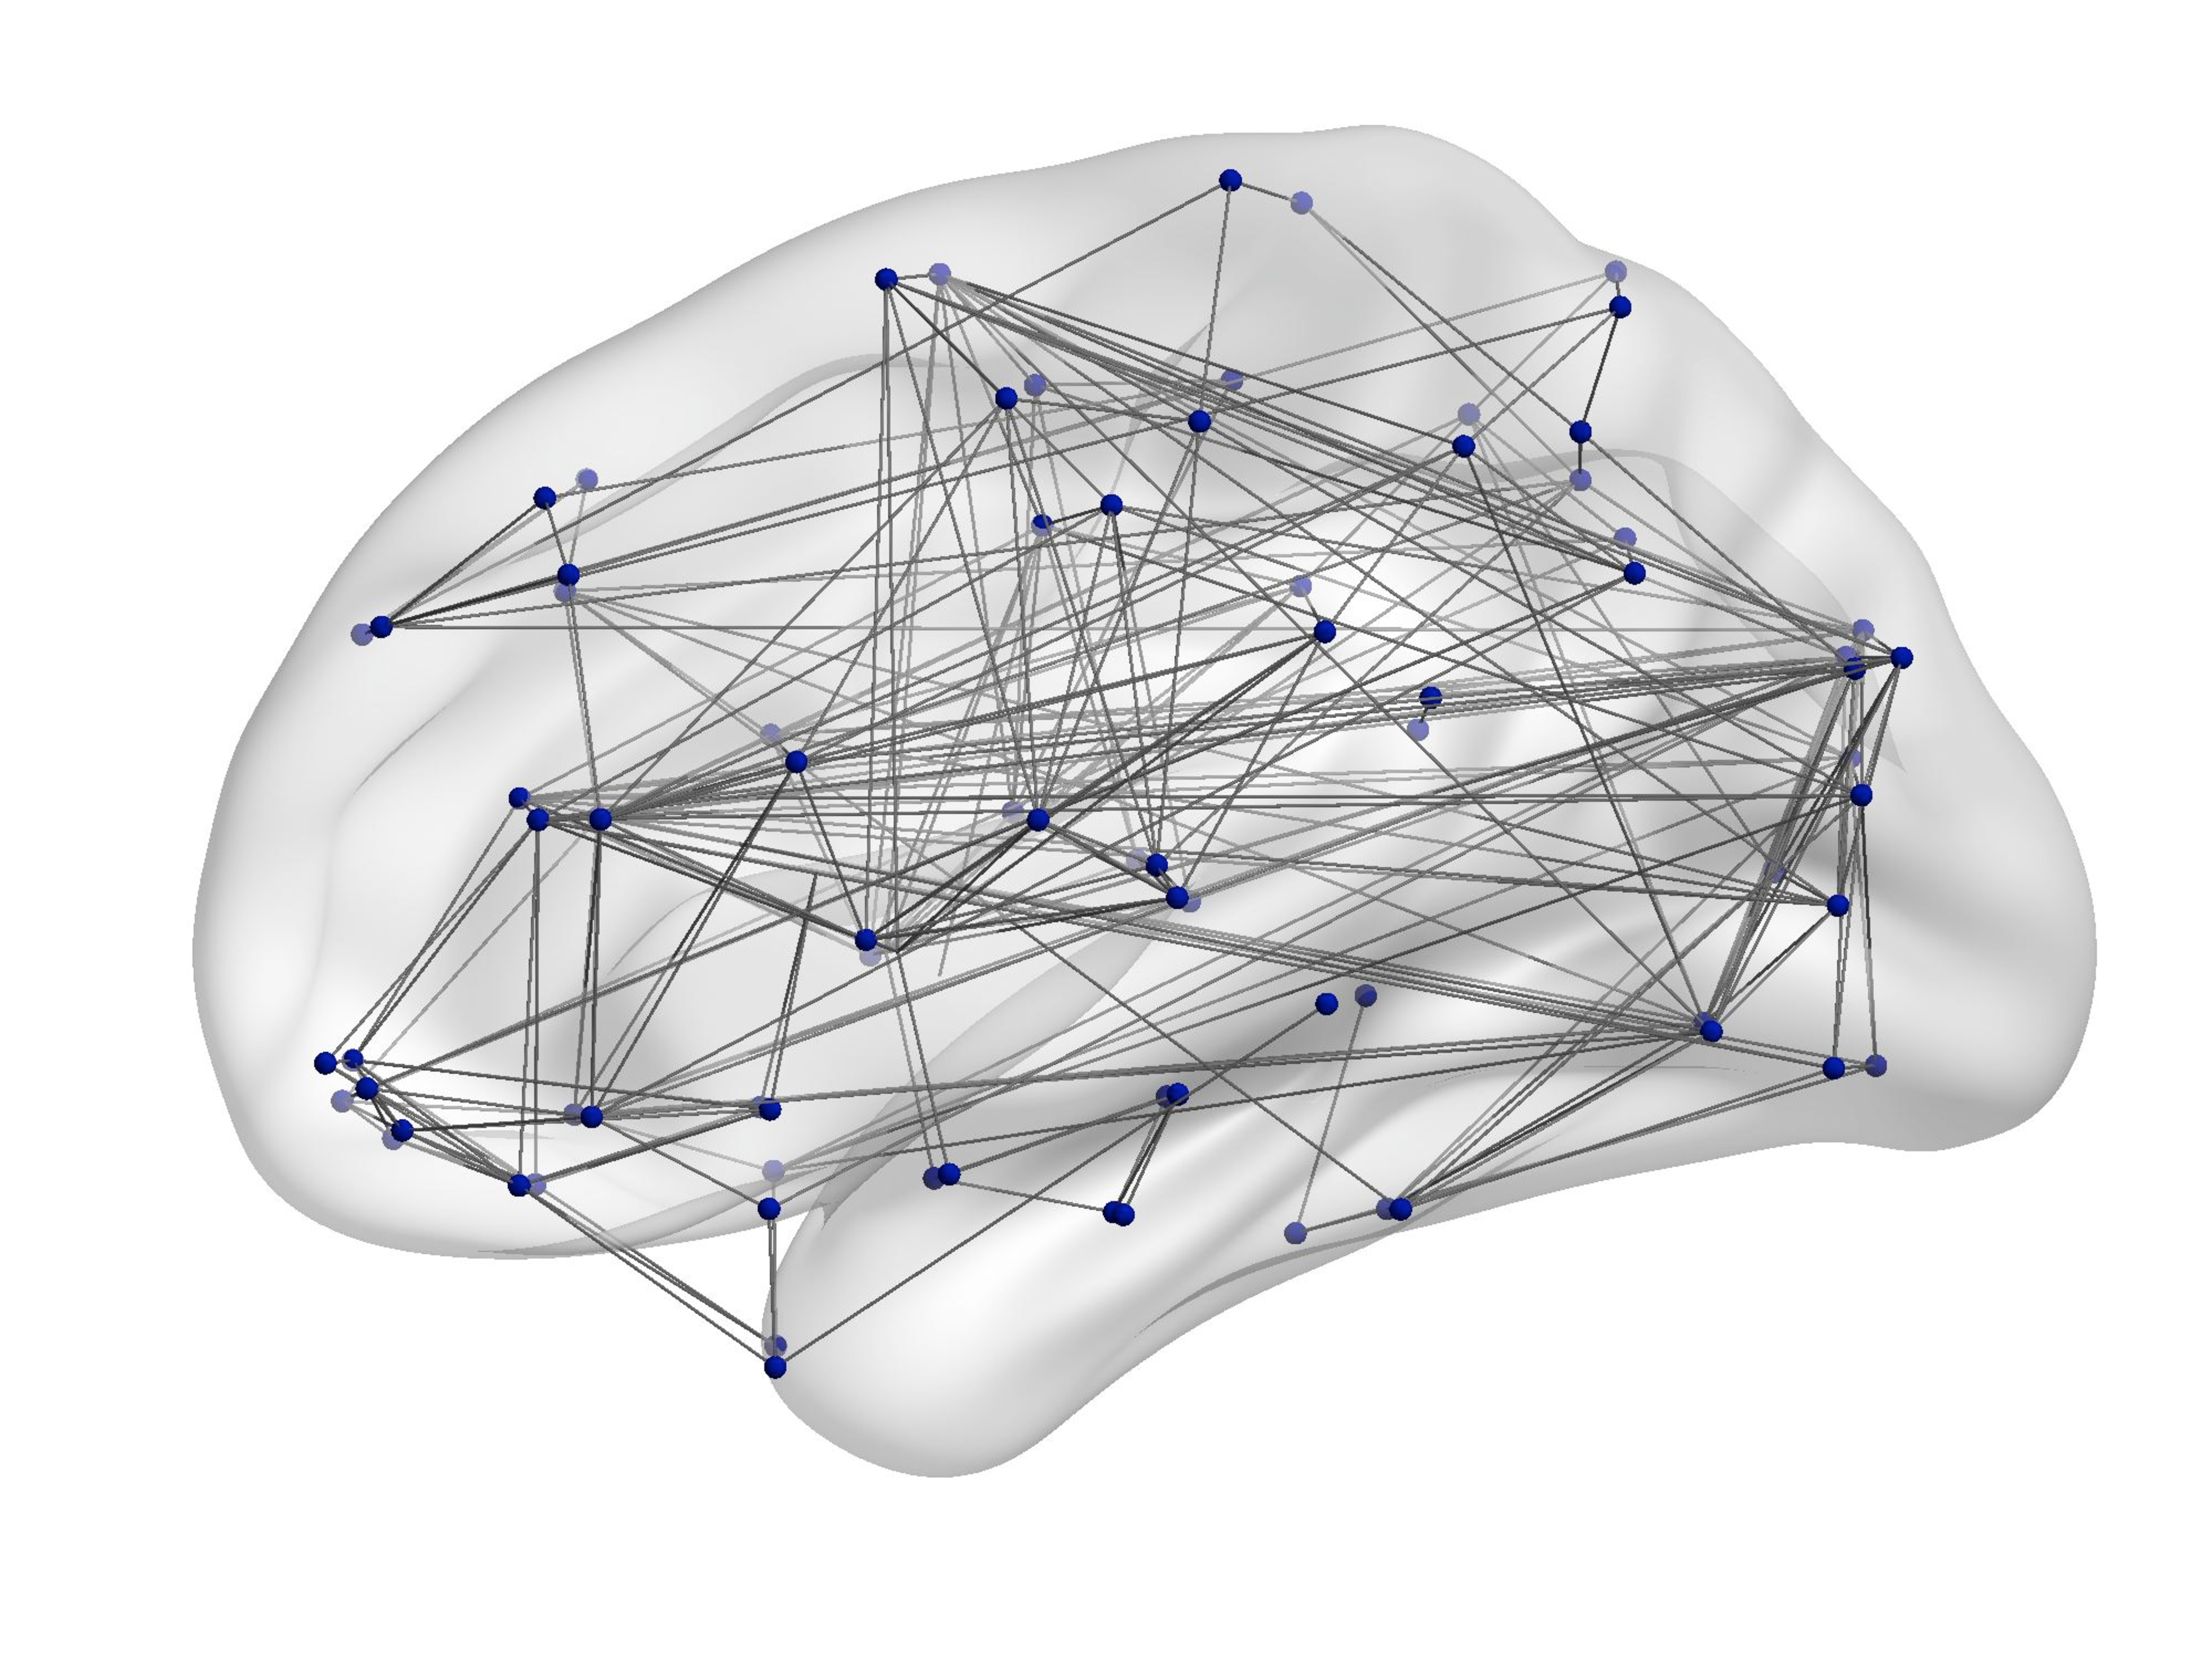
\includegraphics[width=0.4\textwidth,height=0.2\textheight,keepaspectratio]{figures/Young-Central-Sagittal.pdf}
    }
 \hfill
    \subfigure[Frontal lesioning in elderly\label{subfig-2:dummy}]{%
      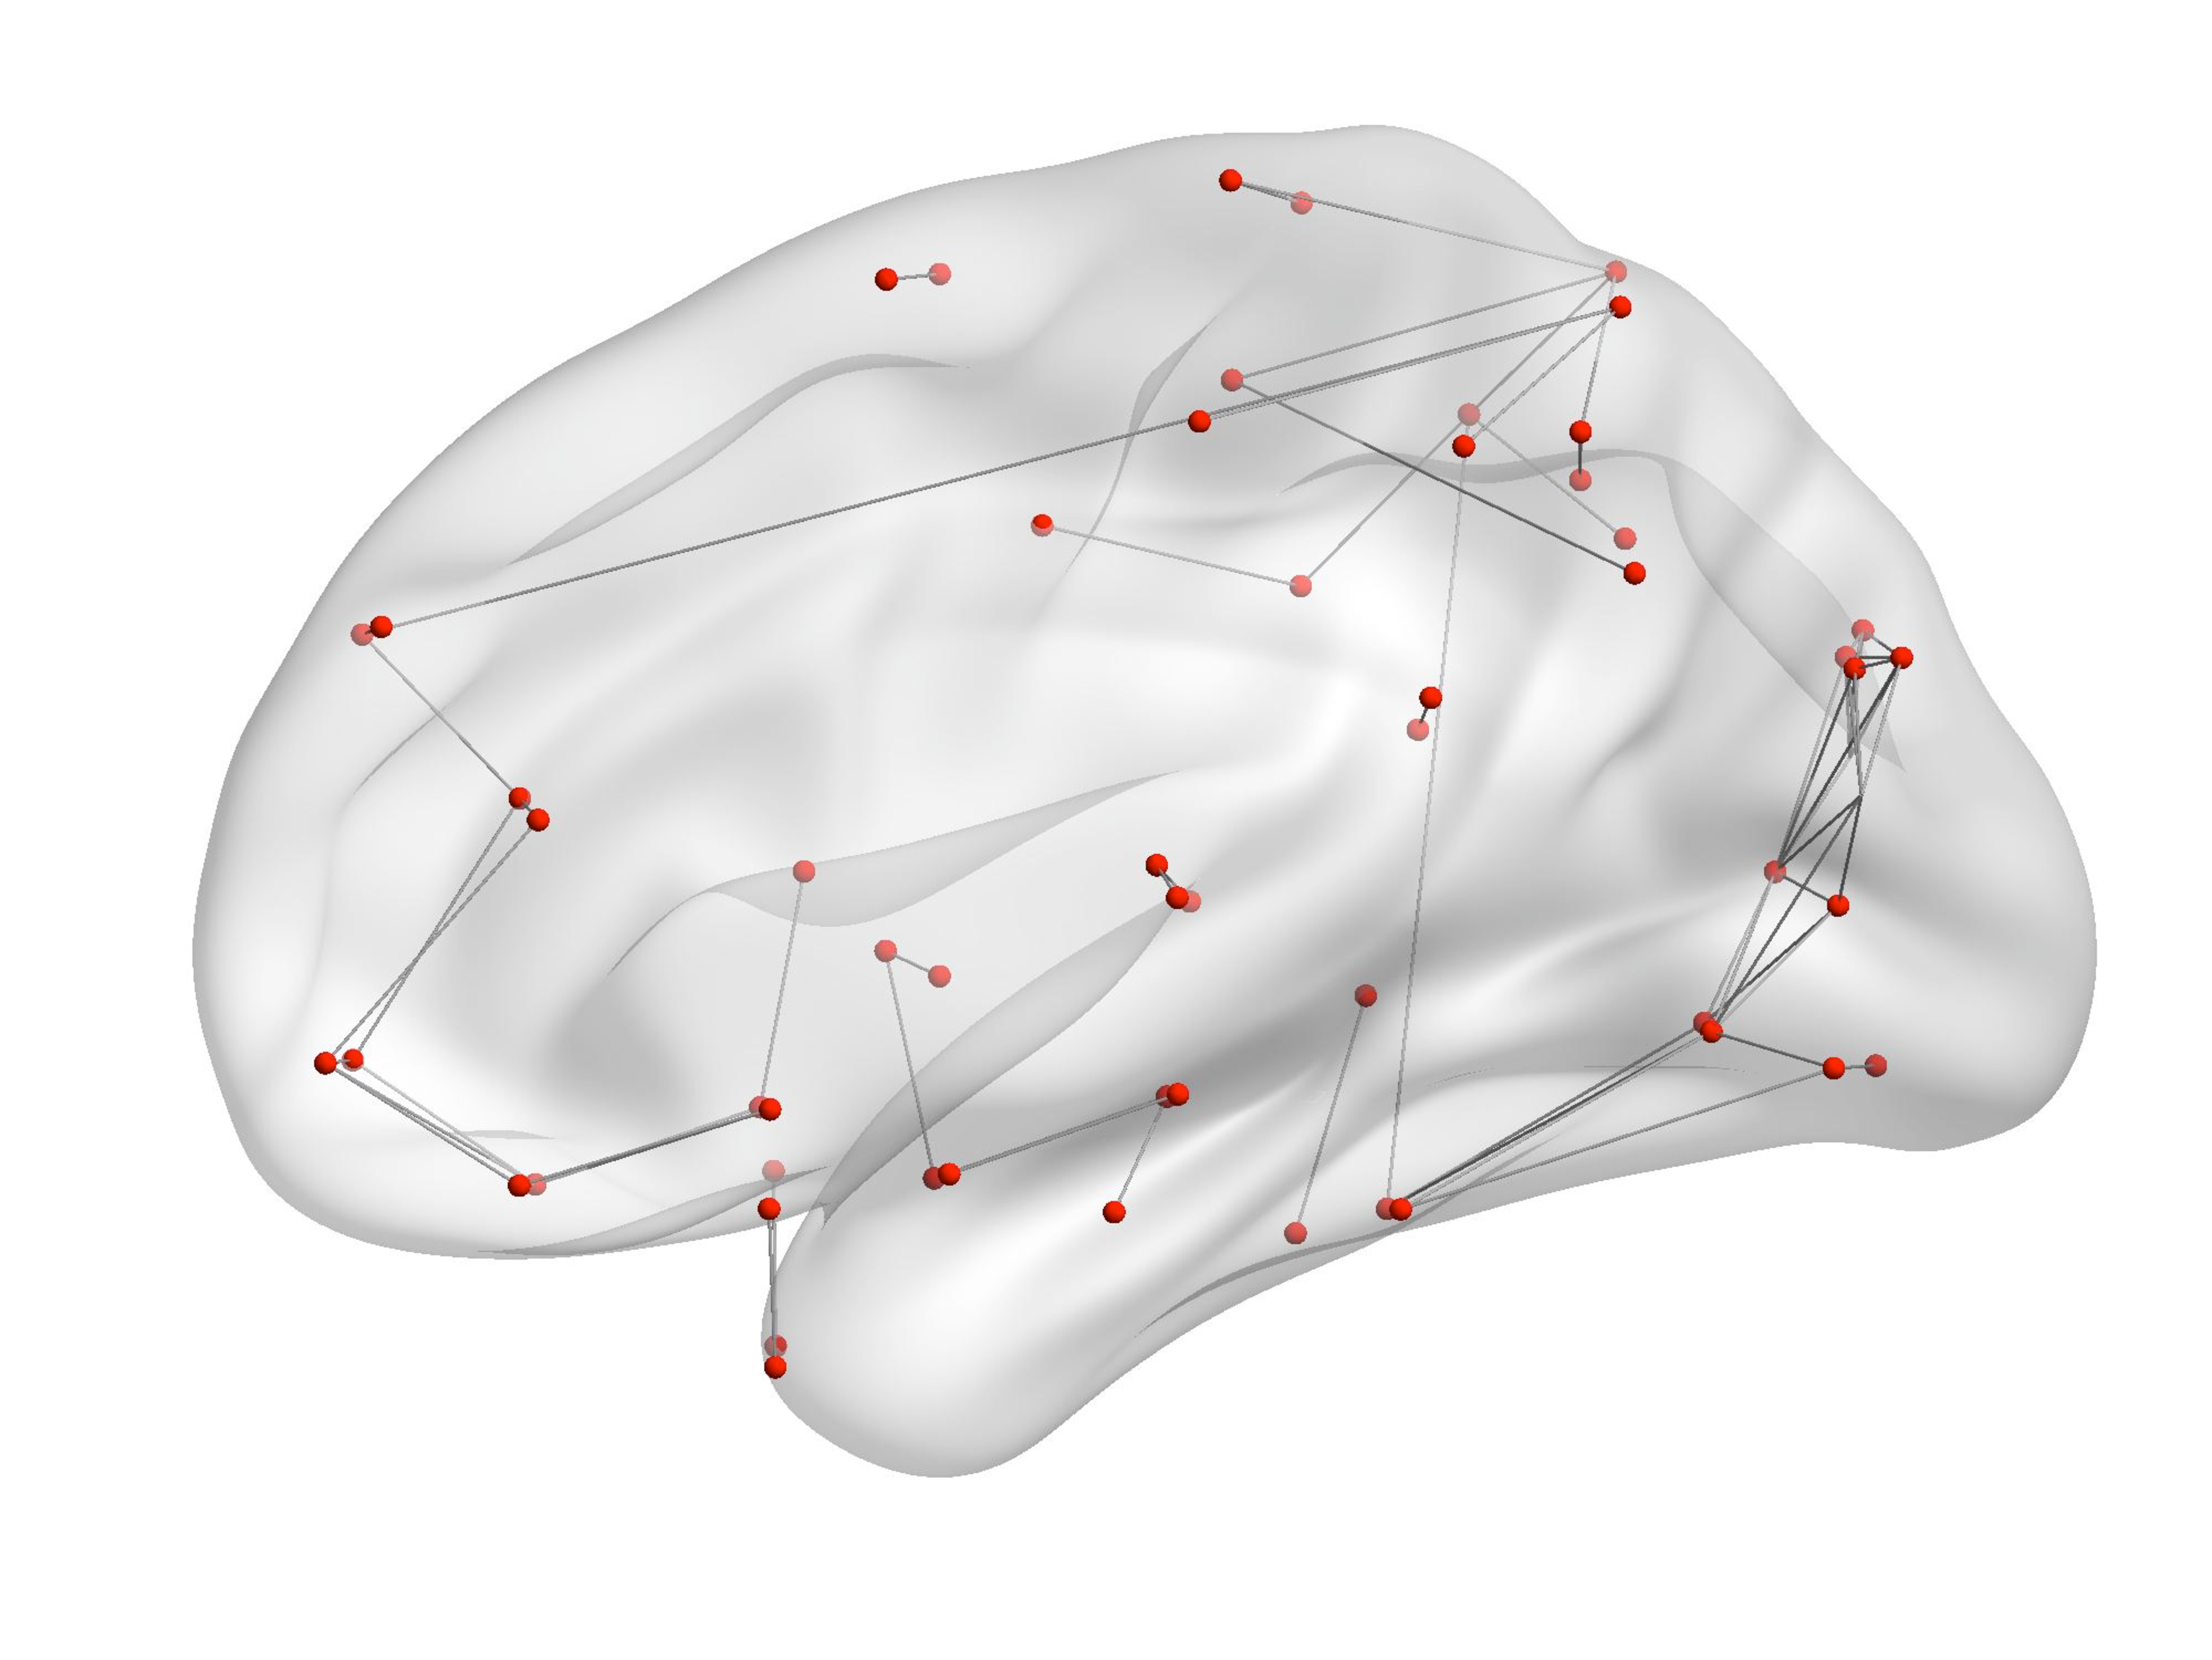
\includegraphics[width=0.4\textwidth,height=0.2\textheight,keepaspectratio]{figures/Old-Frontal-Sagittal.pdf}
    }  
 
    \subfigure[Limbic lesioning in young \label{subfig-1:dummy}]{%
      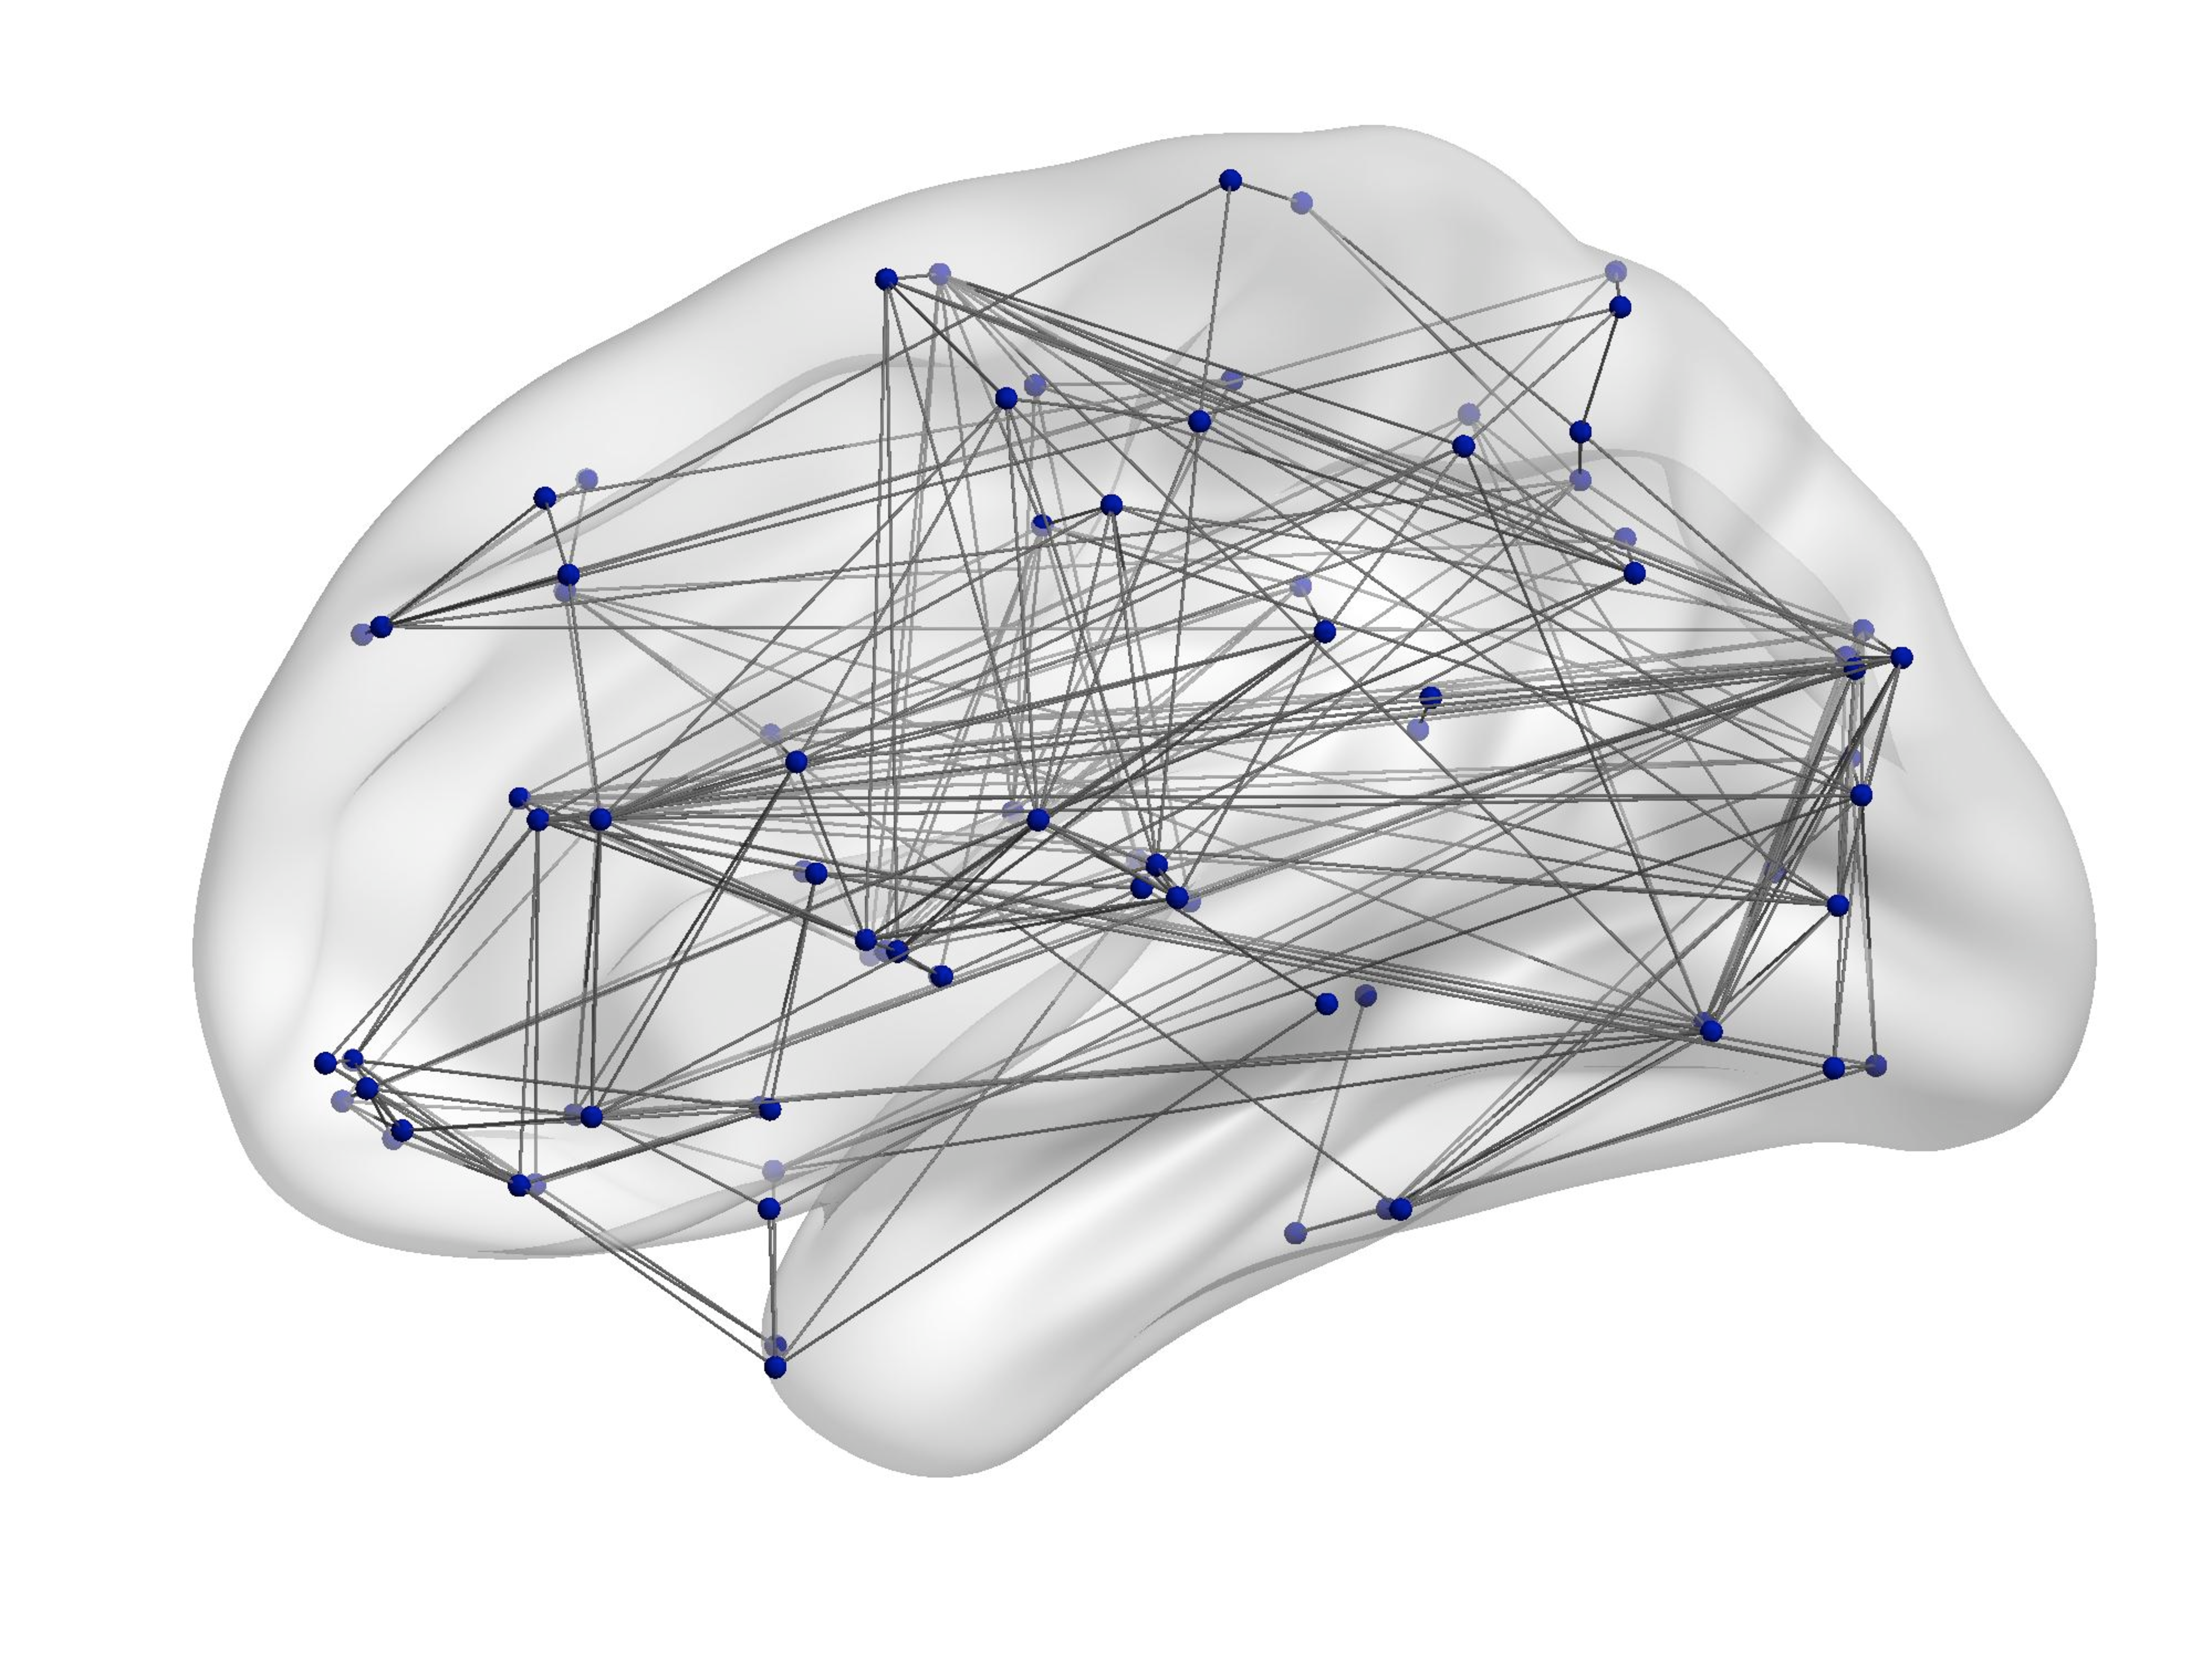
\includegraphics[width=0.4\textwidth,height=0.2\textheight,keepaspectratio]{figures/Young-Limbic-Sagittal.pdf}
    }
 \hfill
    \subfigure[Limbic lesioning in elderly \label{subfig-2:dummy}]{%
      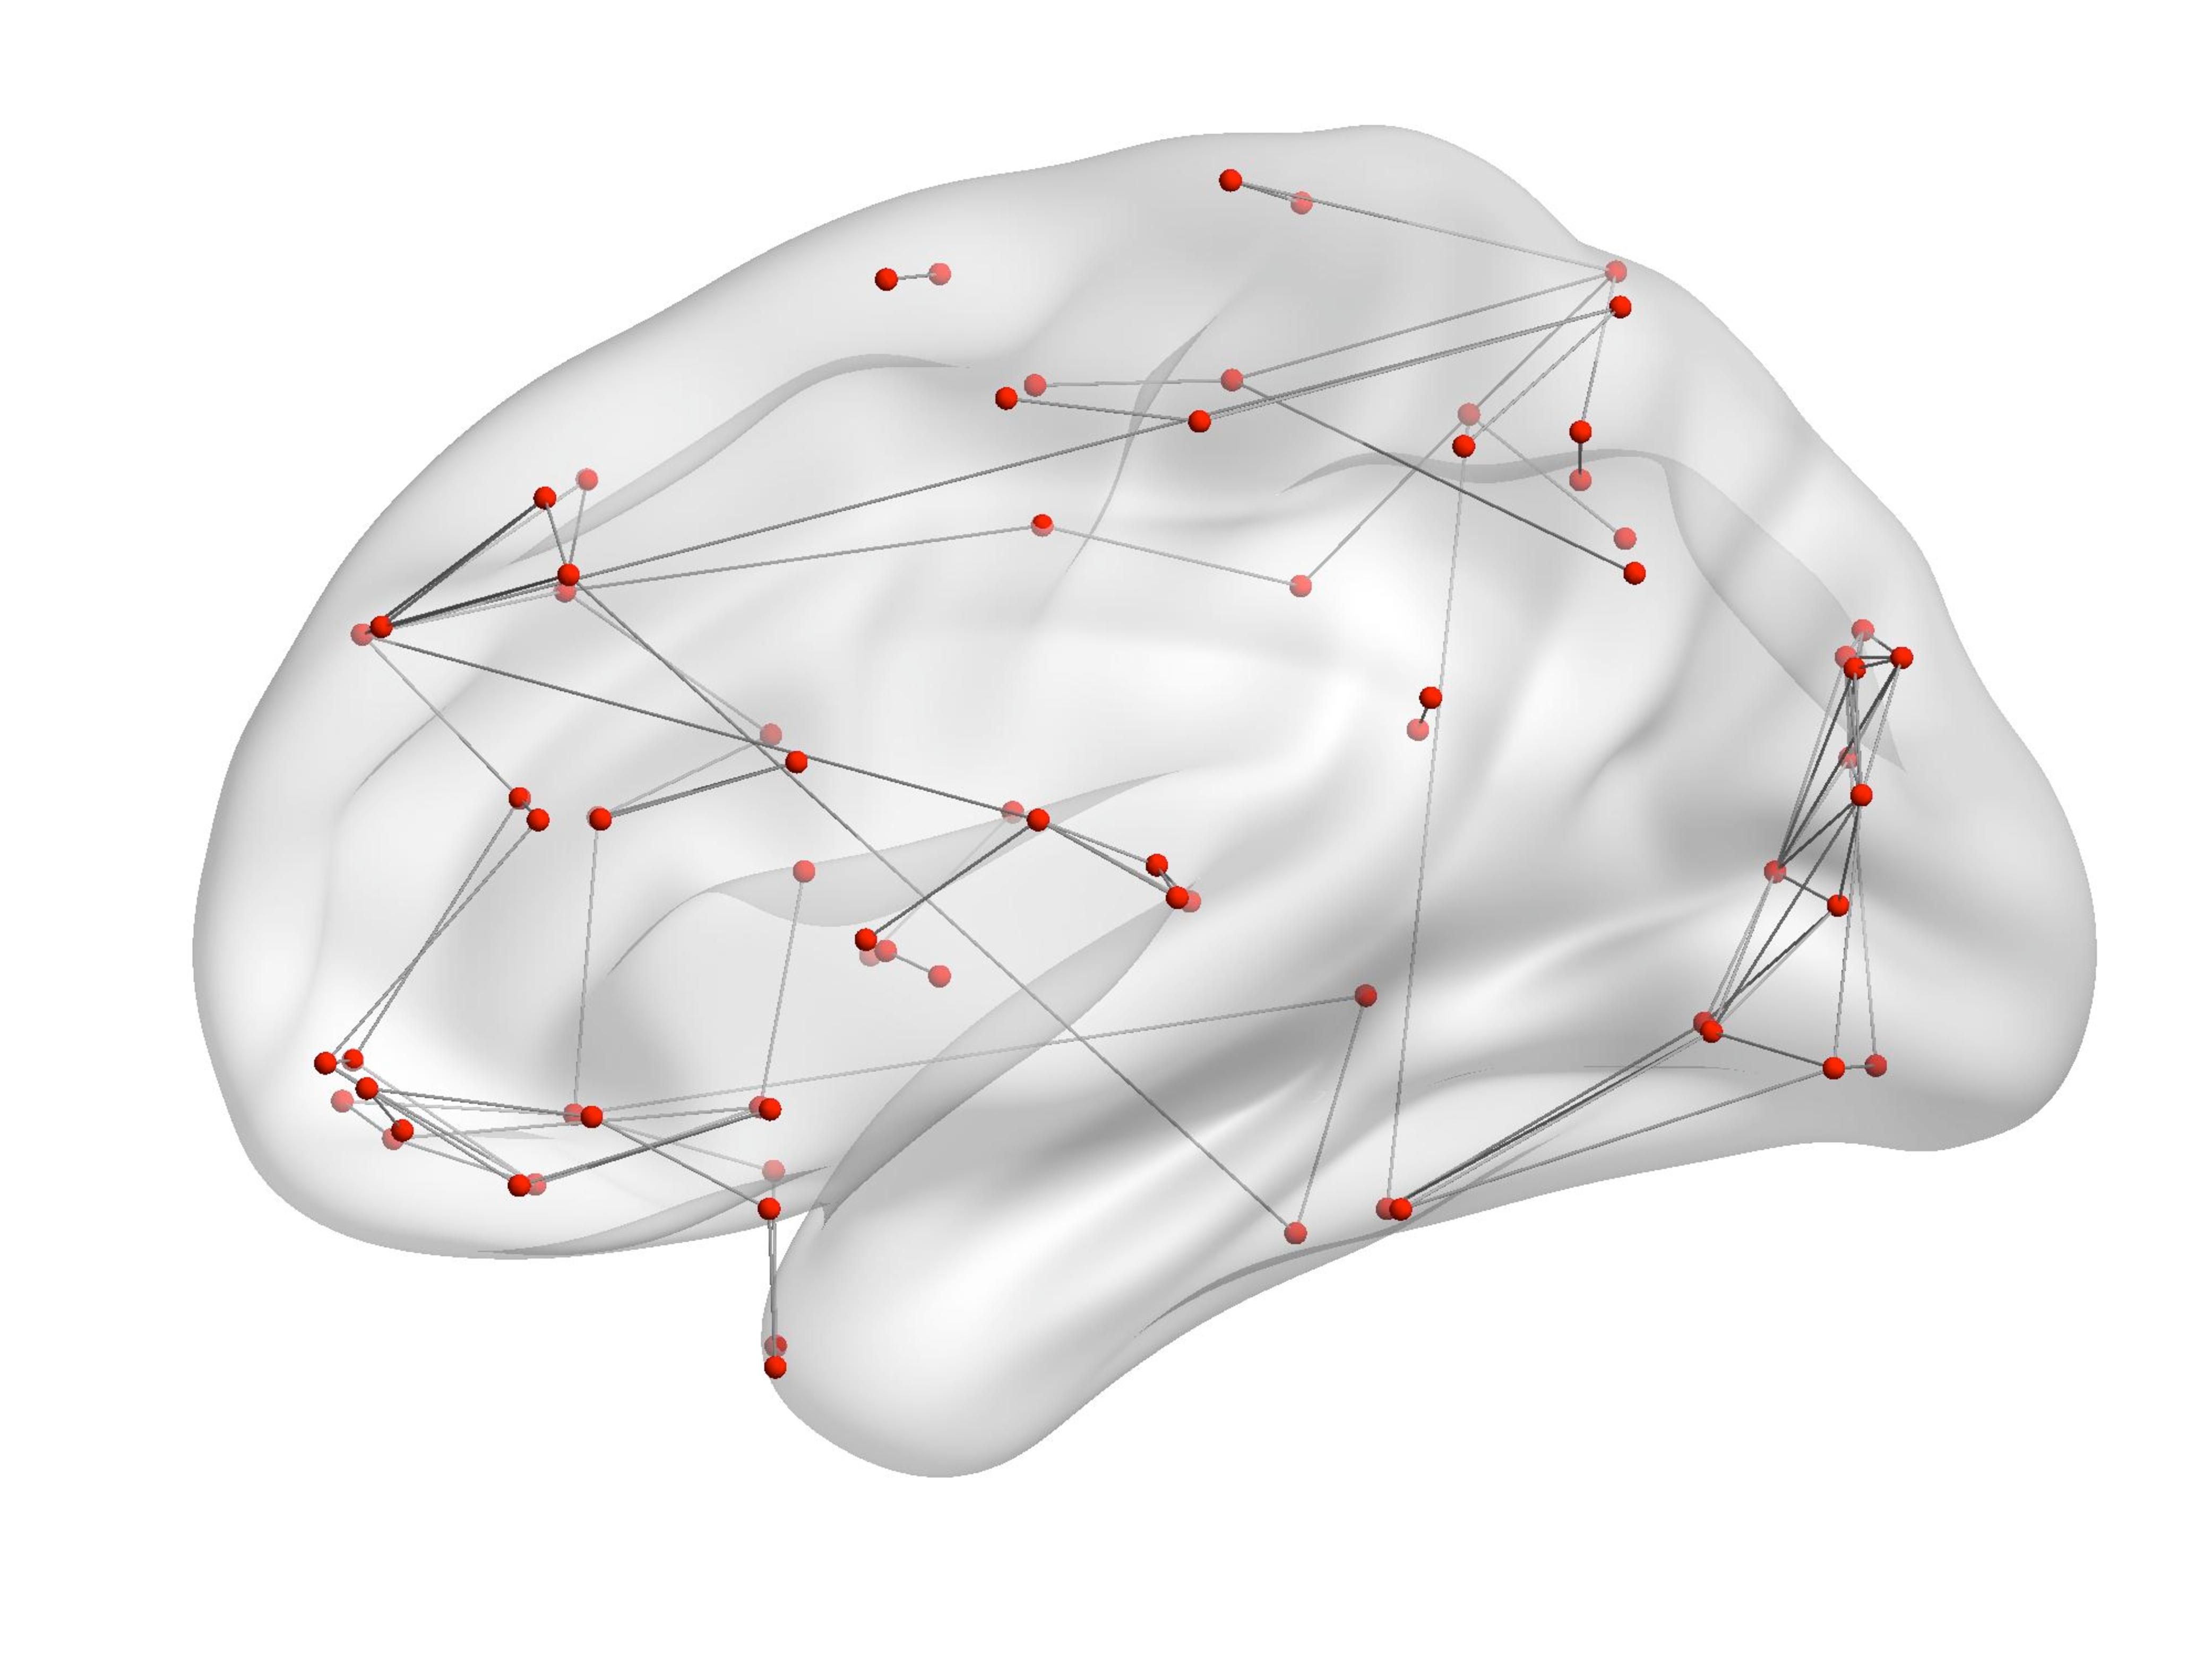
\includegraphics[width=0.4\textwidth,height=0.2\textheight,keepaspectratio]{figures/Old-Limbic-Sagittal.pdf}
    }        
    \label{fig:targetbn}
  \end{figure} 


\begin{table}[!htbp]
\centering%
\caption{The table shows the efficiency loss after the disconnection of different brain structures in both conditions. Interestingly, the reduction in efficiency is not always more pronounced in the elder condition. For example, the disconnection of the central structures (caudate nucleus, putamen, pallidum and thalamus) triggers a larger efficiency disruption in young than in old individuals. A similar situation, larger efficiency loss in young compared old condition, also occurs with the disconnection of the limbic structures (hippocampus, parahippocampus and amygdala) and the occipital lobe areas. The table shows the efficiency loss in both young and old condition when target networks are lesioned. The lesion consists on the obliteration of the nodes defined in the second column. The efficiency loss is larger in old adults with the exception of the occipital lobe, the central structures and the limbic structures. The reduction of efficiency in the central structures is particularly interested since in the old condition it yields only a $3.16\%$ reduction in efficiency while in the young condition the efficiency loss for the same lesioning yields a reduction of $23.01\%$.}
% The minor impact of the lesioning of central and limbic structures is conforming with the degradation of of fronto-stratial nework in aging \cite{salami_elevated_2014} and the break-down between the hipicampal regions and the DMN \cite{fjell_brain_2015}}

\begin{tabularx}{\linewidth}{XXXX}
\toprule
Target Brain Structure & AAL regions & Eff.loss Young &Eff.loss Old\\
\midrule
\midrule
DMN & 3 24 25 26 35 36 37 68 61 62 & $19.66\%$& $61.66\%$\\
\midrule
%Visual areas & 43 44 45 46 47 48 49 50 51 52 53 54 55 56 59 60 89 90 & $38.93\%$ & $55.98\%$\\
%\midrule
Frontal Lobe & 1 2 3 4 5 6 7 8 9 10 11 12 13 14 15 16 17 18 51 52 & $42.83\%$& $67.07\%$\\
\midrule
  Temporal Lobe & 37 38 39 40 41 42 55 56 79 80 81 82 83 84 85 86 87 88 89 90 & $33.56\%$& $41\%$\\
      \midrule
      Occipital Lobe & 43 44 45 46 47 48 49 50 51 52 53 54 & $31.71\%$& $30.79\%$\\
	 \midrule      
	 Parietal Lobe & 57 58 59 60 61 62 63 64 65 66 67 68 & $26.65\%$& $45.64\%$\\
	\midrule      
	Insula and cingulate gyrus & 3 24 25 26 35 36 37 68 61 62 & $18.72\%$& $36.91\%$\\
   \midrule     
    Central structures (Caudate nucleus, putamen, pallidum, thalamus) & 71 72 73 74 75 76 77 78 & $23.01\%$& $3.16\%$\\
     \midrule 
     Limbic structures (hippocampus, parahippocampus, amygdala) & 37 38 39 40 41 42 & $9.30\%$& $1.40\%$\\
     \bottomrule
\end{tabularx}
\label{tab:nodesn}
\end{table}


\subsection{Efficiency after target networks lesioning of edges}
\label{ss:edges}
%Lesion of edges
To test the hypothesis that that the relationship between the hippocampus and the DMN tends to break down with age we need to lesion the edges that connect these brain structures rather than nodes as we have done in the previous sections. 
Salami et al. show that \cite{salami_elevated_2014} elevated hippocampal activity at rest may lower the degree to which the hippocampus interacts with other regions during memory tasks, and thus results in memory deficits. However, this view is not uncontested and in \cite{Damoiseaux_2015} it is suggested that connectivity between left and right hippocampus is negatively related to age.
%https://ww4.aievolution.com/hbm1501/index.cfm?do=abs.viewAbs&abs=4088
In our study the efficiency loss produced by the disconnection of the left and the right side of hippocampal and parahippocampal areas does not yield a reduction of efficiency loss since these areas are not connected in the old subjects (Table \ref{tab:edges}) 

We apply the efficiency measure for lesioning of edges and we found no significant effect of age on DMN inter-connectivity ($0.16\%$ of efficiency loss in young subjects and $0.9\%$ in old subjects upon the disconnection of areas in different hemispheres).   
%Hypothesis testing: Asymmtry
We test the asymmetry hypothesis by which brain activity shows a more balance activity among the two hemispheres with age, that is, the hypothesis predicts that in young individuals brain activity is more asymmetric than in old individuals. To test it, we lesion sequentially the left and the right hemisphere and we calculate the efficiency loss for each case. The asymmetry hypothesis summons that in young individuals the difference in efficiency loss for disconnecting the hemispheres is expected to be larger than in the old condition. Aging thus, tries to compensate the reduction of activity level, for example in the DMN, by balancing the activity across the brain. 
%delete all odds, delete all even, Distance
We see, on the contrary, that if one of the two hemispheres is entirely lesioned, the efficiency loss in young adults is $75.32\%$ when the left side is lesioned and $77.01\%$ when the right side is gone. 
%The difference is 0.0169.
In old subjects, the lesioining of the right side has a more pronounced impact in the efficiency loss, $91.21\%$ for the removal of the right side and $70.89\%$ for the removal of the left side. 
%The differece is 0.2032.  
This result is consistent with the HAROLD (hemispheric asymmetry reduction in older adults) model proposed by  
Cabeza \cite{cabeza_aging_2002}. The difference in efficiency loss in old subjects after entire hemispheral disconnection 
is 10 times larger ($\sim 20\%$) than in the young subjects ($\sim 2\%$) indicates that old subjects are more sensitive or less robust to unilateral disruptions because aging process tend to reduce hemispheric asymmetry.
We hypothesize that a process of de-differentiation may be a key mechanism to explain age-related hemispheric asymmetry reductions. As it was already mentioned in section \ref{ss:single}  the efficiency loss triggered by the disconnection of brain areas is more stereotypical (less differentiated) in the elder condition than in young condition.

\begin{table}[!htbp]
\centering%
\caption{Efficiency loss caused by the deletion of edges that connect brain regions in young and elder conditions. For example DMN-DMN is the deletion of the edges that connect the right and the side of the DMN, DMN-HC the edges that connect DMN and HC, including parahippocampal areas}
\begin{tabularx}{\linewidth}{XXX}
\toprule
Network-Network Edges disconnection & Eff.loss Young & Eff.loss Old\\
\midrule
\midrule
DMN-DMN & $0.64\%$& $0.99\%$\\
\midrule
HC-HC & $1.43\%$& $0.45\%$\\
\midrule
HC-DMN & $0.16\%$& $0\%$\\
\midrule
Frontal-Stratium & $0.37\%$& $0\%$\\
\bottomrule
\end{tabularx}
\label{tab:edges}
\end{table}


\section{Discussion}
\label{discussion}

The objective of this work is to study network robustness i.e., resilience to
perturbations, in resting state functional connectivity networks in young and elderly conditions.
The literature reviewed here suggests that graph-based network
analyses are capable of uncovering system-level changes associated with
aging in the resting brain. 
%A new theoretical framework to investigate network invariance under perturbation and how it is affected by internally driven processes such as aging is provided.
We have analyzed the functional connectivity in resting state using a perturbational approach consisting on either the systematic removal of single nodes and the removal of entire networks of interest such as the DMN and others. We have computed the loss in network efficiency upon the lesioning of brain areas.
%Random removal 1 node
Our results expand previous works on the study of robustness of
structural brain networks. %
Interestingly, we find that the distribution of network efficiency in the young and the elder condition show very different signatures. This is consistent with existing evidence \cite{meunier_age-related_2009} that both young and elderly conditions show non random modularity and that normal aging brain is associated with changes in modularity \cite{song_age-related_2014}.

The functional resting state network in young adults is more robust to random node removal than in elder subjects. The efficiency loss in young subjects, upon the removal of single nodes is always below the $5\%$, while in the elder condition the removal of individual nodes may yield a dramatic reduction of the network efficiency (max $32.87\%$).
The young adults are, thus, more robust to random deletion of single nodes. However, when the lesioning is focused in specific brain networks rather than single regions, the efficiency loss for young subjects is in occassions higher than when the same damage is done in old subjects. For example, the disconnection of the occipital lobe, limbic structures and central structures yield larger efficiency loss in the young condition. This result is compatible with previous studies in normal healthy aging that show an increase in functional connectivity in the sensorimotor network and a decrease in resting state networks, including the DMN \cite{song_age-related_2014}.
The continuum decrease in DMN functional connectivity found from normal aging to mild cognitive impairment and to Alzheimer's disease (AD) can be quantitatively studied. The lowering of DMN activity is associated with better performance on attention-demanding tasks, and DMN hyperactivity is being related to negative rumination and depression \cite{whitfield-gabrieli_default_2012}.    

We replicate the common finding that older subjects present reduced functional connectivity compared to young adults \cite{sala-llonch_changes_2014}. Healthy normal aging is associated with cognitive decline and the functional disconnection observed here and other studies might play an important role \cite{ferreira_resting-state_2013}, \cite{dennis_functional_2014}.  
We observe largest values of efficiency loss in old adults compared to young adults in the Default-Mode-Network and the frontal lobe (Table \ref{tab:nodesn})
This is consistent with the compensation hypothesis in healthy aging which states that older adults brains compensate for the overall functional deficits by increasing the activity levels in some areas. In this view, the DMN is a highly susceptible system in healthy aging \cite{betzel_changes_2014}, \cite{onoda_decreased_2012}.  Increased activity is being observed in frontal regions as a reorganization process mediated by healthy normal aging \cite{cabeza_aging_2002}, \cite{park_adaptive_2009}   

Can efficiency loss be used as a predictor of brain network differential activity? 
To address this question further work is we needed in order to properly address the compatibility of informational efficiency with non parametric classifiers. 
Vergun et al. \cite{vergun_characterizing_2013} applied a Support Vector Machine (SVM) linear classifier to rs-fMRI data in order to compare age-related differences in four of the major functional brain networks: the default, cingulo-opercular, fronto-parietal, and sensorimotor. 
With this method they detected "connectivity hubs", or nodes with the most significant features that influenced age classification. 
%The best predictors of age based on SVM are not coincident with the best predictors in age using the efficiency loss method. 
%YOSOLO atlas boundaries agreement meta studies classifier with metatalases 
%, and replicate our results with different imaging techniques
%Hypothesis testing: SVM

With this work we expect to pave the way for future works to establish a link between pathological lesions and
the topological centrality and efficiency measures provided here. Informational efficiency measures may also shed light on the dynamics and control of resting state networks in mental disorders. A natural continuation of this work is to incorporate a translational outlook to, for example, investigate whether hubs of human brain networks are more likely to be anatomically abnormal than non-hubs in many brain disorders \cite{crossley_hubs_2014}.
This perturbational approach can also be extended to study the interplay between network efficiency and brain metabolic demand, aiming to identify pathological signatures for early diagnosis in neurodegenerative disorders. The network dynamics associated with different conditions -normal healthy aging, mild cognitive impairment, Alzheimer's disease etc.- can be simulated with the same or similar type of functional intervention proposed here. Interventions other than disconnecting regions of interest or entire subnetworks from the whole brain, may include stress simulations induced by impairment of structural, functional or both connectivity patterns in multimodal imaging models. The computational lesioning of brain foci holds promise for systemic understanding of compensatory mechanisms and other network mechanisms e.g., cascade and contagion effects, under normal and pathological conditions.   

\bibliographystyle{plain}
\bibliography{/Users/jagomez/Eclipse/workspace/bibliojgr/bibliojgr}
%\bibliography{bibliojgr}

\end{document}